\documentclass[english,floatsintext,man]{apa6}

\usepackage{amssymb,amsmath}
\usepackage{ifxetex,ifluatex}
\usepackage{fixltx2e} % provides \textsubscript
\ifnum 0\ifxetex 1\fi\ifluatex 1\fi=0 % if pdftex
  \usepackage[T1]{fontenc}
  \usepackage[utf8]{inputenc}
\else % if luatex or xelatex
  \ifxetex
    \usepackage{mathspec}
    \usepackage{xltxtra,xunicode}
  \else
    \usepackage{fontspec}
  \fi
  \defaultfontfeatures{Mapping=tex-text,Scale=MatchLowercase}
  \newcommand{\euro}{€}
\fi
% use upquote if available, for straight quotes in verbatim environments
\IfFileExists{upquote.sty}{\usepackage{upquote}}{}
% use microtype if available
\IfFileExists{microtype.sty}{\usepackage{microtype}}{}

% Table formatting
\usepackage{longtable, booktabs}
\usepackage{lscape}
% \usepackage[counterclockwise]{rotating}   % Landscape page setup for large tables
\usepackage{multirow}		% Table styling
\usepackage{tabularx}		% Control Column width
\usepackage[flushleft]{threeparttable}	% Allows for three part tables with a specified notes section
\usepackage{threeparttablex}            % Lets threeparttable work with longtable

% Create new environments so endfloat can handle them
% \newenvironment{ltable}
%   {\begin{landscape}\begin{center}\begin{threeparttable}}
%   {\end{threeparttable}\end{center}\end{landscape}}

\newenvironment{lltable}
  {\begin{landscape}\begin{center}\begin{ThreePartTable}}
  {\end{ThreePartTable}\end{center}\end{landscape}}




% The following enables adjusting longtable caption width to table width
% Solution found at http://golatex.de/longtable-mit-caption-so-breit-wie-die-tabelle-t15767.html
\makeatletter
\newcommand\LastLTentrywidth{1em}
\newlength\longtablewidth
\setlength{\longtablewidth}{1in}
\newcommand\getlongtablewidth{%
 \begingroup
  \ifcsname LT@\roman{LT@tables}\endcsname
  \global\longtablewidth=0pt
  \renewcommand\LT@entry[2]{\global\advance\longtablewidth by ##2\relax\gdef\LastLTentrywidth{##2}}%
  \@nameuse{LT@\roman{LT@tables}}%
  \fi
\endgroup}


\ifxetex
  \usepackage[setpagesize=false, % page size defined by xetex
              unicode=false, % unicode breaks when used with xetex
              xetex]{hyperref}
\else
  \usepackage[unicode=true]{hyperref}
\fi
\hypersetup{breaklinks=true,
            pdfauthor={},
            pdftitle={An information-seeking account of eye movements during signed and spoken language comprehension},
            colorlinks=true,
            citecolor=blue,
            urlcolor=blue,
            linkcolor=black,
            pdfborder={0 0 0}}
\urlstyle{same}  % don't use monospace font for urls

\setlength{\parindent}{0pt}
%\setlength{\parskip}{0pt plus 0pt minus 0pt}

\setlength{\emergencystretch}{3em}  % prevent overfull lines

\ifxetex
  \usepackage{polyglossia}
  \setmainlanguage{}
\else
  \usepackage[english]{babel}
\fi

% Manuscript styling
\captionsetup{font=singlespacing,justification=justified}
\usepackage{csquotes}
\usepackage{upgreek}

 % Line numbering
  \usepackage{lineno}
  \linenumbers


\usepackage{tikz} % Variable definition to generate author note

% fix for \tightlist problem in pandoc 1.14
\providecommand{\tightlist}{%
  \setlength{\itemsep}{0pt}\setlength{\parskip}{0pt}}

% Essential manuscript parts
  \title{An information-seeking account of eye movements during signed and spoken
language comprehension}

  \shorttitle{Information-seeking eye movements}


  \author{Kyle MacDonald\textsuperscript{1}, Virginia Marchman\textsuperscript{1}, Anne Fernald\textsuperscript{1}, \& Michael C. Frank\textsuperscript{1}}

  % \def\affdep{{"", "", "", ""}}%
  % \def\affcity{{"", "", "", ""}}%

  \affiliation{
    \vspace{0.5cm}
          \textsuperscript{1} Stanford University  }

  \authornote{
    Correspondence concerning this article should be addressed to Kyle
    MacDonald, 450 Serra Mall, Stanford, CA 94306. E-mail:
    \href{mailto:kylem4@stanford.edu}{\nolinkurl{kylem4@stanford.edu}}
  }


  \abstract{Understanding grounded language involves mapping the incoming linguistic
signal onto the visual world. Information that is gathered through
visual fixations can facilitate comprehension. But how do listeners
decide what visual information to gather and at what time? Here, we
propose that listeners flexibly adapt their gaze to seek visual
information from social partners that supports language understanding.
We present evidence for our account using three case studies of eye
movements during real-time language processing. First, compared to
children learning spoken English (n=80), young ASL-learners (n=30)
delayed gaze shifts away from a language source, were more accurate and
produced a smaller proportion of nonlanguage-driven shifts. Second,
English-speaking adults (n=24) produced fewer random gaze shifts when
processing serially-presented text compared to processing spoken
language. Finally, English-speaking preschoolers (n=39) and adults
(n=31) delayed the timing of gaze shifts away from a speaker while
processing speech in noisy environments. This delay resulted in
gathering more visual information and more accurate responding. These
results provide converging evidence that listeners adapt their gaze to
seek supportive visual information from their social partners.}
  \keywords{eye movements; language comprehension; information-seeking; speech in
background noise; American Sign Language \\

    \indent Word count: X
  }





\begin{document}

\maketitle

\setcounter{secnumdepth}{0}



\hypertarget{introduction}{%
\section{Introduction}\label{introduction}}

Extracting meaning from language represents a formidable challenge for
young language learners. Consider that even in the simple case of
understanding grounded, familiar language (e.g., \enquote{look at the
ball}), the listener must integrate linguistic and non-linguistic
information from continuous streams of input. Moreover, language unfolds
within dynamic interactions where there is often insufficient
information to figure out what is being said, and yet the listener must
decide how best to respond. Despite these challenges, even young
children are capable of mapping language to the world quite efficiently,
shifting visual attention to a named object in a scene within hundreds
of milliseconds upon hearing the name of an object (Allopenna, Magnuson,
\& Tanenhaus, 1998; Spivey, Tanenhaus, Eberhard, \& Sedivy, 2002;
Tanenhaus, Spivey-Knowlton, Eberhard, \& Sedivy, 1995). How do young
listeners interpret language despite noisy input and their developing
processing capabilities?

One solution is for children to integrate multiple sources of
information to constrain the set of possible interpretations (MacDonald
\& Seidenberg, 2006; McClelland \& Elman, 1986). Under this interactive
account, listeners comprehend words by partially activating several
candidates that are consistent with incoming perceptual information.
Then, as more information arrives, words that do not match the
perceptual signal are no longer considered, and words that are more
consistent become strongly activated until a single interpretation is
reached (see McClelland, Mirman, and Holt (2006) for a review).
Critically, information from multiple sources -- e.g., the linguistic
signal, visual world, and conceptual knowledge -- mutually influence one
another to shape interpretation. For example, if a speaker's mouth
movements suggest one sound while their acoustic output indicates
another, the interaction results in the listener perceiving a third,
intermediate sound (\enquote{McGurk effect}) (MacDonald \& McGurk,
1978). Other research shows that listeners will use information in the
visual scene to help parse syntactically ambiguous utterances (Tanenhaus
et al., 1995).

Thus, information gathered from the visual world can serve as a useful
information for comprehending language. But the incoming linguistic
signal is ephemeral, meaning that listeners must quickly decide how to
direct their gaze to informative locations. Consider a speaker who asks
you to \enquote{Pass the salt} in a noisy restaurant. Here,
comprehension could be supported by looks that better encode the objects
in the scene (e.g., the type of food she is eating), or by looks to the
speaker (e.g., reading her lips or the direction of her gaze). A second
interesting case is the processing a visual-manual language such as
American Sign Language (ASL). In this context, signers have to decide
when to look away from a language source, a choice that is inherently
risky because shifting gaze reduces visual access to subsquent
linguistic information.

These examples highlight how eye movements during grounded language
comprehension can be characterized as an active decision-making process
that seeks to maximize the return on language-relevant information over
time. In this work, we pursue this idea and propose that listeners are
sensitive to the value of different fixation behaviors for the goal of
grounded language understanding. We hypothesize that even young children
can flexibly adapt the dynamics of their gaze to seek higher value
visual information. At the core of this account is the idea that eye
movements are shaped by a coupling between sensorimotor constraints and
the quality of language-relevant information in the visual world.

Our account is inspired by ideas from several, rich research traditions.
First, work on language-mediated visual attention showing rapid
interactions between visual attention and language (Allopenna et al.,
1998; Tanenhaus et al., 1995). Second, research on vision in everyday
tasks shows that people allocate fixations to \emph{goal-relevant}
locations -- e.g., an upcoming obstacle while walking (Hayhoe \&
Ballard, 2005). Finally, work on multisensory integration showing that
listeners leverage multimodal cues (e.g., gestures, facial expressions,
mouth movements) to support communication. In the following sections, we
briefly review each of these literatures to motivate our
information-seeking account of eye movements in social, grounded
language comprehension.

\hypertarget{vision-language-interactions-during-language-comprehension}{%
\subsection{Vision-Language interactions during language
comprehension}\label{vision-language-interactions-during-language-comprehension}}

Eye movements during language comprehension have provided insight into
the interaction between concepts, language, and visual attention. The
majority of this work has used the Visual World Paradigm (VWP) where
listeners' eye movements are recorded at the millisecond timescale while
processing language and looking at a set of objects (see Salverda,
Brown, and Tanenhaus (2011) for a review). Crucially, these analyses
rely on the fact that people will initiate gaze shifts to named
referents with only partial information, in contrast to waiting until
the end of a cognitive process (Gold \& Shadlen, 2000). Thus, the
timecourse of eye movements provides a window onto how and when people
integrate information to reach an interpretation of the incoming
linguistic signal.

A classic finding using the VWP shows that listeners will rapidly shift
visual attention upon hearing the name of an object (\enquote{Pick up a
beaker.}) in the visual scene with a high proportion of shifts occurring
soon after the target word begins (Allopenna et al., 1998). Moreover,
adults tended to look at phonological onset-competitor (a beetle) early
in the target noun, suggesting that they had activated multiple
interpretations and resolved ambiguity as the stimulus unfolded. These
behavioral results fall out of predictions made by interactive models of
speech perception where information from multiple sources is integrated
to constrain language understanding (McClelland et al., 2006).

The visual world can also constrain the set of plausible interpretations
of language (Dahan \& Tanenhaus, 2005; Yee \& Sedivy, 2006). For
example, Altmann and Kamide (2007) showed that people will allocate more
looks to an empty wine glass as compared to a full beer glass upon
hearing the past tense verb \enquote{has drunk.} They propose that
anticipatory eye movements reflect the influence of the visual
information in a scene activating a multi-featured, conceptual
representation prior to the arrival of the linguistic signal (see also
Huettig and Altmann (2005)).

In addition to work on adult psycholinguistics, the VWP has been useful
for studying developmental change in language comprehension skill in
children. Researchers have adapted the task to measure the timing and
accuracy of children's gaze shifts as they look at two familiar objects
and listen to simple sentences naming one of the objects (Fernald,
Zangl, Portillo, \& Marchman, 2008; Venker, Eernisse, Saffran, \&
Weismer, 2013). Such research finds that children, like adults, shift
gaze to named objects occur soon after the auditory information is
sufficient to enable referent identification. Moreover, individual
differences in the speed and accuracy of eye movements predict
vocabulary growth and later language and cognitive outcomes (Fernald,
Perfors, \& Marchman, 2006; Marchman \& Fernald, 2008; Rigler et al.,
2015). Finally, the VWP has illustrated interesting developmental
parallels and differences between children's language processing in
different populations, including sign language (MacDonald, LaMarr,
Corina, Marchman, \& Fernald, 2018), bilingualism (Byers-Heinlein,
Morin-Lessard, \& Lew-Williams, 2017), and children with cochlear
implants (Schwartz, Steinman, Ying, Mystal, \& Houston, 2013).

\hypertarget{goal-based-accounts-of-eye-movements-in-everyday-tasks}{%
\subsection{Goal-based accounts of eye movements in everyday
tasks}\label{goal-based-accounts-of-eye-movements-in-everyday-tasks}}

The majority of the work on language-driven visual attention has used
eye movements as an index of the underlying interaction between
linguistic and visual information. This approach reflects a somewhat
passive construal of how people allocate visual attention during
language comprehension. In contrast, goal-based accounts of vision start
from the idea that eye movements reflect an active information-gathering
process where visual fixations are driven by task goals (Hayhoe \&
Ballard, 2005).

Under this account, people allocate visual attention to reduce
uncertainty about the world and maximize the expected future reward. For
example, Hayhoe and Ballard (2005) review evidence that people fixate on
locations that are most helpful for their current goal (an upcoming
obstacle) as opposed to other aspects of a visual scene that might be
more salient (a flashing light). Moreover, other work shows that people
gather task-specific information via different visual routines as they
become useful for their goals. For example, Triesch et al 2003 found
that people were much less likely to gather and store visual information
about the size of an object when it was not relevant to the task of
sorting and stacking the objects.

Hayhoe and Ballard (2005)'s review also highlights the role of learning
gaze patterns. They point out that visual routines are developed over
time, and it is only when a task becomes highly-practiced that people
allocate fewer looks to less relevant parts of the scene. For example,
Shinoda, Hayhoe, and Shrivastava (2001) show that drivers, with
practice, learn to spread visual attention more broadly at intersections
to better detect stop signs. Other empirical work shows that the visual
system rapidly learns to use temporal regularities in the environment to
control the timing of eye movements to detect goal-relevant events
(Hoppe \& Rothkopf, 2016). Moreover, the timing of eye movements in
these tasks often occur before an expected event (i.e., anticipatory),
suggesting that gaze patterns reflect an interaction between people's
expectations, information available in the visual scene, and their task
goals.

Recent theoretical work has argued for a stronger link between
goal-based perspectives and work on eye movements during language
comprehension. For example, Salverda et al. (2011) highlight the
immediate relevance of visual information with respect to the goal of
language understanding, suggesting that listeners' goals should be a key
predictor of fixation patterns. Moreover, they point out that factors
such as the difficulty of executing a real world task should change
decisions about where to look during language comprehension. One example
of starting from a goal-based approach comes from Nelson and Cottrell
(2007)' study of gaze patterns during category learning. Nelson and
Cottrell (2007) modeled eye movements as a type of question-asking about
features of a concept and showed that the dynamics of eye movements
changed as participants became more familiar with the novel concepts
their gaze patterns shift from exploratory to efficient, suggesting that
fixations changed as a function of learning goals during the task.

In the current studies, the goal-based model of eye movements predicts
that gaze during language comprehension should adapt to the processing
context. That is, listeners should change the timing and location of eye
movements when fixation locations become more useful for comprehension.
This proposal dovetails with a growing body of research that explores
the effects of multisensory (e.g., gesture, prosody, facial expression
and body movement) integration on language perception and comprehension.

\hypertarget{language-perception-as-multisensory-integration}{%
\subsection{Language perception as multisensory
integration}\label{language-perception-as-multisensory-integration}}

Language comprehension does not just involve a single stream of
linguistic information. Instead, face-to-face communication provides the
listener with access to a set of multimodal cues that can facilitate
comprehension. There is a growing emphasis on studying language as a
multimodal and multisensory process (for a review, see Vigliocco,
Perniss, and Vinson (2014)). For example, empirical work shows that when
gesture and speech provide redundant cues to meaning, people are faster
to process the information and make fewer errors (Kelly, Özyürek, \&
Maris, 2010). Moreover, developmental work shows that parents use visual
cues such as gesture and eye gaze to help structure language
interactions with their children (Estigarribia \& Clark, 2007). Finally,
from a young age, children also produce gestures such as reaches and
points to share attention with others to achieve communicative goals
(Liszkowski, Brown, Callaghan, Takada, \& De Vos, 2012).

Additional support for multisensory processing comes from work on
audiovisual speech perception, showing how spoken language perception is
shaped by visual information coming from a speaker's mouth. In a review,
Peelle and Sommers (2015) point out that mouth movements provide a clear
indication of when someone has started to speak, which cues the listener
to allocate additional attention to the speech signal. Moreover, a
speaker's mouth movements convey information about the phonemes in the
acoustic signal. For example, visual speech information distinguishes
between consonants such as \textbf{/b/} vs. \textbf{/d/} and place of
articulation can help a listener differentiate between words such as
\enquote{cat} or \enquote{cap.} Finally, classic empirical work shows
comprehension benefits for audiovisual speech compared to auditory- or
visual-only speech, especially in noisy listening contexts (Erber,
1969).

In sum, the work on multisensory processing shows that both auditory and
visual information interact to shape language perception. These results
parallel the claims of the interactive models of language processing
reviewed earlier and suggest that visual information should be
considered as an input to language comprehension (MacDonald \&
Seidenberg, 2006; McClelland et al., 2006). Finally, these results
highlight the value of studying language comprehension during
face-to-face communication, where listeners can choose to look at their
social partners to gather language-releveant visual information.

\hypertarget{the-present-studies}{%
\subsection{The present studies}\label{the-present-studies}}

The studies reported here characterize language processing as a
multimodal, goal-based, and social phenomenon. We propose an
information-seeking account of eye movements during grounded language
comprehension in both signed and spoken language. The timing of gaze
shifts reflect a maximization of gathering language-relevant visual
information from a speaker balanced with fixating on surrounding visual
scene. We draw on models of eye movements as active decisions that
gather information to achieve reliable interpretations of incoming
language and test predictions of our account using three case studies of
processing sign language, serially-presented text, and spoken language
in noisy environments. These cases represent a broad sampling of
contexts that share a key feature: The interaction between the listener
and environment changes the value of fixating on the source of language
to support comprehension.

A secondary goal of this work was to test whether children and adults
would show similar patterns of gaze adaptation. Recent developmental
work shows that, like adults, preschoolers will flexibly adjust how they
interpret ambiguous sentences (e.g., \enquote{I had carrots and
\emph{bees} for dinner.}) by integrating information about the
reliability of the incoming perceptual information with their
expectations about the speaker (Yurovsky, Case, \& Frank, 2017). While
children's behavior paralleled adults, they relied more on top-down
expectations about the speaker perhaps because their perceptual
representations were noisier. These developmental differences provide
insight into how children succeed in understanding language despite
having partial knowledge of word-object mappings.

The structure of the paper is as follows. First, we compare children and
adult's eye movements while processing signed vs.~spoken language. Then,
we present a study of adults' eye movements while processing
serially-presented text as compared to spoken language. Finally, we
compare children and adults' gaze patterns while they process speech in
noisy vs.~clear auditory environments. The key behavioral prediction is
that both children and adults will adapt the timing of their eye
movements to facilitate word recognition. We hypothesized that as a
language source provides higher value visual information, listeners
should prioritize fixations to their social partner, and would be (a)
slower to shift gaze away, which in turn would lead to (b) more accurate
responding and (c) fewer nonlanguage-driven eye movements to the
\emph{rest} of the visual world.

Before describing the studies, it is worth motivating our analytic
approach. To quantify evidence for our predictions, we analyze the
accuracy and reaction times (RTs) of listeners' initial gaze shifts
after hearing the name of an object. The timescale of this analysis is
milliseconds and focuses on a single decision within a series of
decisions about where to look during language processing. We chose this
approach because first shifts are rapid decisions driven by accumulating
information about the identity of the named object and thus provide a
window onto changes in the underlying dynamics of how listeners
integrate linguistic and visual information. Finally, by focusing our
analysis on a specific, discrete choice, we could leverage cognitive
models of decision making developed over the past forty years (the Drift
Diffusion Model (2008)) that quantify changes in the underlying
psychological processes that generate fixation decisions.

\hypertarget{experiment-1}{%
\section{Experiment 1}\label{experiment-1}}

Experiment 1 provides an initial test of our information seeking
account. We compared eye movements of children learning American Sign
Language to children learning a spoken language using parallel real-time
language comprehension tasks where children processed familiar sentences
(e.g., \enquote{Where's the ball?}) while looking at a simplified visual
world with three fixation targets (a center stimulus that varied by
condition, a target picture, and a distracter picture; see Figure
~\ref{fig:trio-stim}). The spoken language data are a reanalysis of
three unpublished data sets, and the ASL data are reported in MacDonald
et al. (2018). Our primary question of interest is whether processing a
sign language like ASL would increase the value of fixating on the
language source and decrease the value of generating exploratory,
nonlanguage-driven shifts even after the disambiguation point in the
linguistic signal. If ASL learners are sensitive to the cost of shifting
gaze away from a signer, then they would show evidence of prioritizing
accuracy over and above speed of shifting gaze to the named object.

\hypertarget{analysis-plan}{%
\subsection{Analysis plan}\label{analysis-plan}}

To quantify changes in the process of generting eye movements we use
three analyses. First, we present behavioral analyses of the timecourse
of looking to each area of interest (AOI), along with analyses of First
Shift Accuracy and Reaction Time (RT). RT corresponds to the latency of
shifting gaze away from the central stimulus to either object measured
from the onset of the target noun.\footnote{All reaction time
  distributions were trimmed to between zero and two seconds and RTs
  were modeled in log space.} Accuracy corresponds to whether
participants' first gaze shift landed on the target or the distracter
object. It is important to note that this analysis of accuracy does not
focus on the amount of time spent looking at the target vs.~the
distracter image -- a measure typically used in analyses of the Visual
World Paradigm. We chose to focus primarily on first shifts to provide a
window onto changes in the underlying dynamics of information gathering
decisions. All analysis code can be found in the online repository for
this project: \url{https://github.com/kemacdonald/speed-acc}.

We used the \texttt{rstanarm} (Gabry \& Goodrich, 2016) package to fit
Bayesian mixed-effects regression models. The mixed-effects approach
allowed us to model the nested structure of our data -- multiple trials
for each participant and item, and a within-participants manipulation --
by including random intercepts for each participant and item, and a
random slope for each item and noise condition. We used Bayesian
estimation to quantify uncertainty in our point estimates, which we
communicate using a 95\% Highest Density Interval (HDI). The HDI
provides a range of credible values given the data and model. Finally,
to estimate age-related differences, we fit two types of models: (1) age
group (adults vs.~children) as a categorical predictor and (2) age as a
continuous predictor (measured in days) within the child sample.

Next, we present the two model-based analyses. The goal of these models
is to move beyond a description of the data and map behavioral
differences in eye movements to underlying psychological variables. The
Exponetially Weighted Moving Average (EWMA) models changes in the
tendency to generate random gaze shifts as a function of RT
(Vandekerckhove \& Tuerlinckx, 2007). For each RT, the model generates
two values: a \enquote{control statistic} (CS, which captures the
running average accuracy of first shifts) and an \enquote{upper control
limit} (UCL, which captures the pre-defined limit of when accuracy would
be categorized as above guessing). Here, the CS is an expectation of
random shifting to either the target or the distracter image
(nonlanguage-driven shifts), or a Bernoulli process with probability of
success 0.5. As RTs get slower, we assume that participants have
gathered more information and should become more accurate
(language-driven), or a Bernoulli process with probability success
\textgreater{} 0.5. Using this model, we can quantify the proportion of
gaze shifts that were language-driven as opposed to guessing.

Finally, following Vandekerckhove and Tuerlinckx (2007), we selected
shifts categorized as language-driven by the EWMA and fit a hierarchical
Bayesian Drift-Diffusion Model (HDDM). The DDM quantifies differences in
the underlying decision process that lead to different patterns of
behavior. The model assumes that people accumulate noisy evidence in
favor of one alternative with a response generated when the evidence
crosses a pre-defined decision threshold. We chose to implement a
hierarchical Bayesian version of the DDM using the HDDM Python package
(Wiecki, Sofer, \& Frank, 2013) since we had relatively few trials from
child participants and recent simulation studies have shown that the
HDDM approach was better than other DDM fitting methods for small data
sets (Ratcliff \& Childers, 2015). Here, we focus on two parameters of
interest: \emph{boundary separation}, which indexes the amount of
evidence gathered before generating a response (higher values suggest
more cautious responding) and \emph{drift rate}, which indexes the
amount of evidence accumulated per unit time (higher values suggest more
efficient processing).

\hypertarget{methods}{%
\subsection{Methods}\label{methods}}

\hypertarget{participants}{%
\subsubsection{Participants}\label{participants}}

\begin{table}[tbp]
\begin{center}
\begin{threeparttable}
\caption{\label{tab:trio make participants table}Age distributions of children in Experiment 1. All ages are reported in months.}
\begin{tabular}{lllll}
\toprule
Center Stimulus & \multicolumn{1}{c}{Mean} & \multicolumn{1}{c}{Min} & \multicolumn{1}{c}{Max} & \multicolumn{1}{c}{n}\\
\midrule
ASL & 27.90 & 16.00 & 53.00 & 30.00\\
Face & 26.00 & 25.00 & 26.00 & 24.00\\
Object & 31.90 & 26.00 & 39.00 & 40.00\\
Bullseye & 26.10 & 26.00 & 27.00 & 16.00\\
\bottomrule
\end{tabular}
\end{threeparttable}
\end{center}
\end{table}

Table 1 contains details about the age distributions of children in all
of four samples.

\emph{Spoken English samples.} Participants were 80 native, monolingual
English-learning children divided across three samples. Participants had
no reported history of developmental or language delay.

\emph{ASL sample.} Participants were 30 native, monolingual ASL-learning
children (18 deaf, 12 hearing). All children, regardless of hearing
status, were exposed to ASL from birth through extensive interaction
with at least one caregiver fluent in ASL and were reported to
experience at least 80\% ASL in their daily lives. The ASL sample
included a wider age range compared to the spoken English samples
because this is a rare population.

\hypertarget{stimuli}{%
\subsubsection{Stimuli}\label{stimuli}}

\begin{figure}[!t]

{\centering 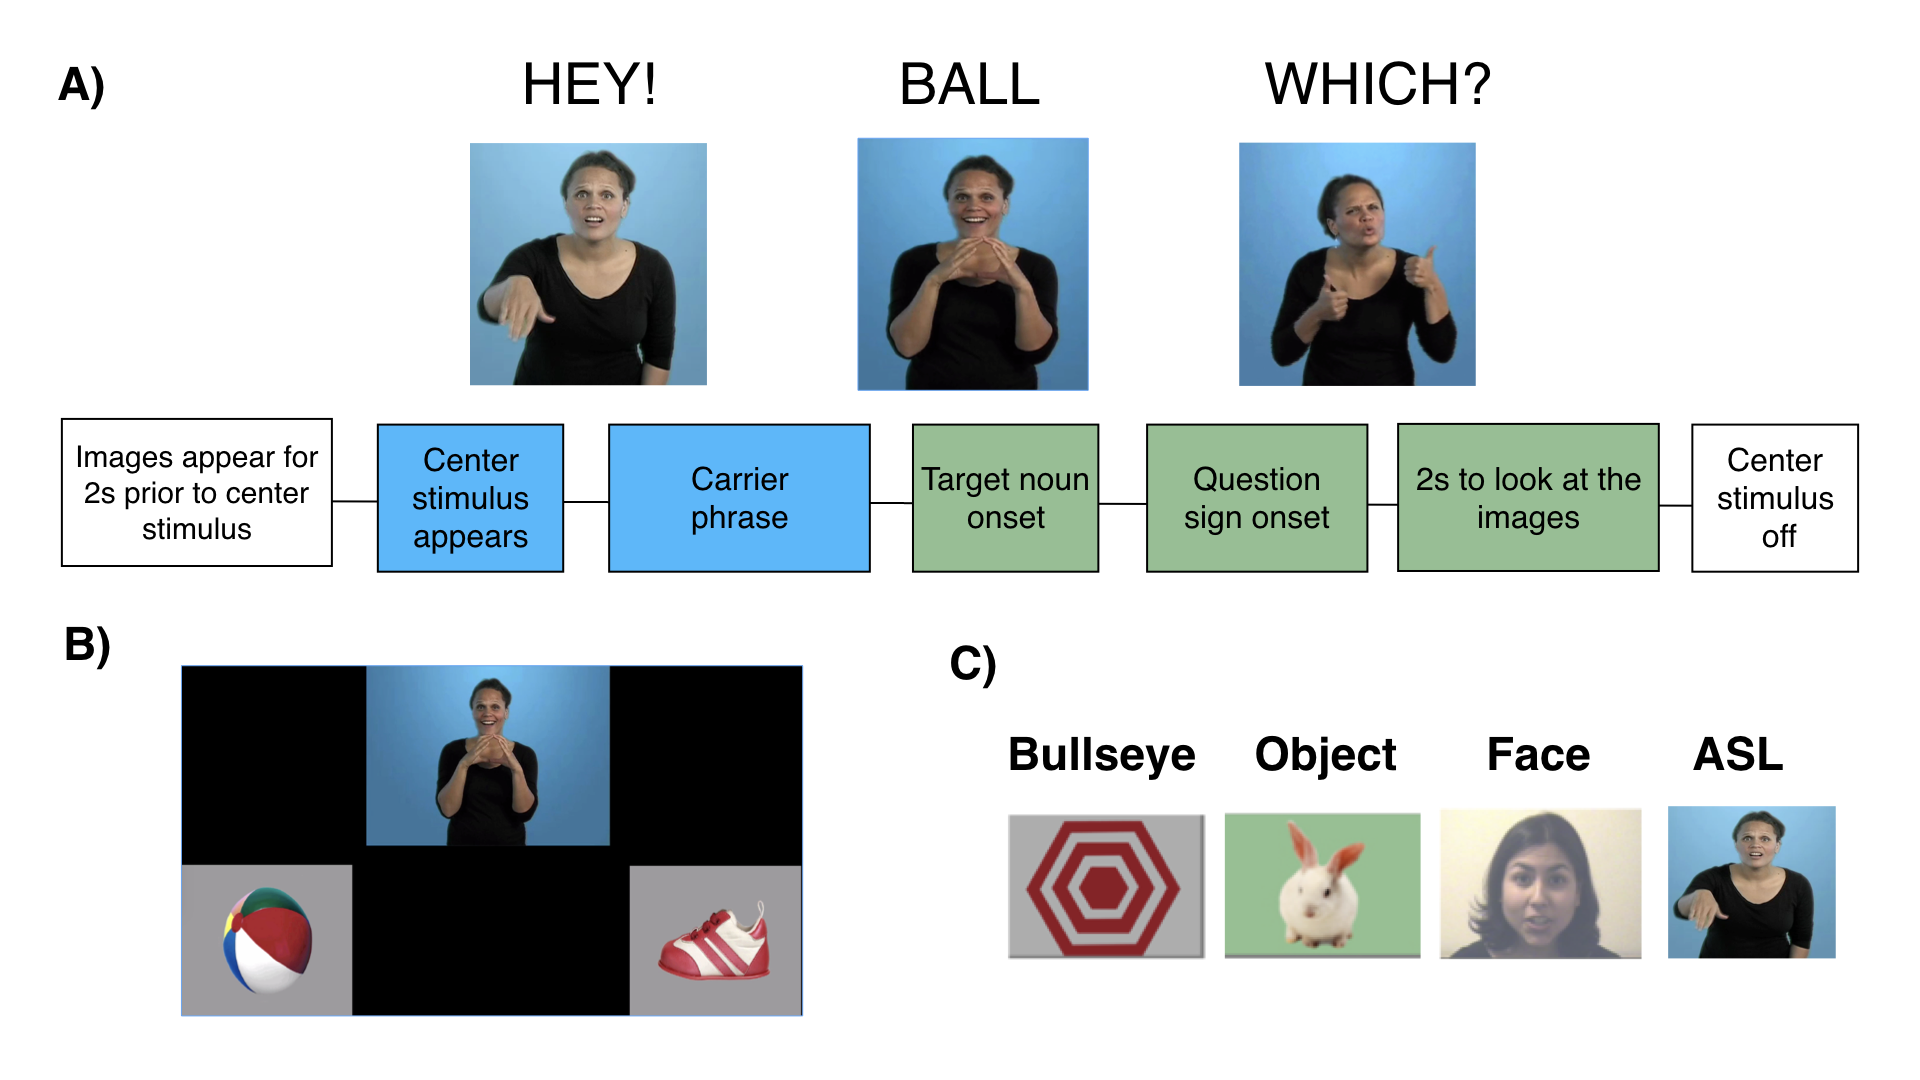
\includegraphics[width=0.9\linewidth]{/Users/kmacdonald/Documents/Projects/SPEED-ACC/paper/journal_submission/figures/figs_output//trio_stimuli} 

}

\caption{Stimuli for Experiments 1 and 2. Panel A shows the timecourse of the linguistic stimuli for a single trial. Panel B shows the layout of the fixation locations for all tasks: the center stimulus, the target, and the distracter. Panel C shows the five center stimulus items: a static geometric shape (Bullseye), a static image of a familiar object (Object), a person speaking (Face), a person signing (ASL), and a serially-presented text display (Text).}\label{fig:trio-stim}
\end{figure}

There are differences between ASL and English question structures.
However, all linguistic stimuli shared the same trial structure:
language to attract participants' attention followed by a sentence
containing a target noun.

\emph{ASL linguistic stimuli.} We recorded two sets of ASL stimuli,
using two valid ASL sentence structures for questions: 1)
Sentence-initial wh-phrase: \enquote{HEY! WHERE {[}target noun{]}?} and
2) Sentence-final wh-phrase: \enquote{HEY! {[}target noun{]} WHERE?} Two
female native ASL users recorded several tokens of each sentence in a
child-directed register. Before each sentence, the signer produced a
common attention-getting gesture. Mean sign length was 1.25 sec, ranging
from 0.69 sec to 1.98 sec.

\emph{English linguistic stimuli.} All three tasks (Object, Bullseye,
and Face) featured the same female speaker who used natural
child-directed speech and said: \enquote{Look! Where's the (target
word)?} The target words were: ball, banana, book, cookie, juice, and
shoe. For the Face task, a female native English speaker was
video-recorded as she looked straight ahead and said, \enquote{Look!
Where's the (target word)?} Mean word length was 0.79 sec, ranging from
0.60 sec to 0.94 sec.

\emph{ASL and English visual stimuli.} The image set consisted of
colorful digitized pictures of objects presented in fixed pairs with no
phonological overlap (ASL task: cat---bird, car---book, bear---doll,
ball---shoe; English tasks: book-shoe, juice-banana, cookie-ball). Side
of target picture was counterbalanced across trials.

\emph{Trial structure.} On each trial, the child saw two images of
familiar objects on the screen for two seconds before the center
stimulus appeared. This time allowed the child to visually explore both
images. Next, the target sentence -- which consisted of a carrier
phrase, target noun, and question sign -- was presented, followed by two
seconds without language to allow the child to respond to the signer's
sentence. The trial structure of the Face, Object, and Bullseye tasks
were highly similar: children were given two seconds to visually explore
the objects prior to the appearance of the center stimulus, then
processed a target sentence, and finally were given two seconds of
silence to generate a response to the target noun.

\hypertarget{design-and-procedure}{%
\subsubsection{Design and procedure}\label{design-and-procedure}}

Children sat on their caregiver's lap and viewed the task on a screen
while their gaze was recorded using a digital camcorder. On each trial,
children saw two images of familiar objects on the screen for two
seconds before the center stimulus appeared (see Figure 1). Then they
processed the target sentence -- which consisted of a carrier phrase, a
target noun, and a question -- followed by two seconds without language
to allow for a response. Participants saw 32 test trials with several
filler trials interspersed to maintain interest.

\emph{Coding.} Participants' gaze patterns were coded (33-ms resolution)
as being fixated on either the center stimulus, one of the images,
shifting between pictures, or away. To assess inter-coder reliability,
25\% of the videos were re-coded. Agreement was scored at the level of
individual frames of video and averaged 98\% on these reliability
assessments.

\hypertarget{results-and-discussion}{%
\subsection{Results and Discussion}\label{results-and-discussion}}

\begin{figure}[!t]

{\centering 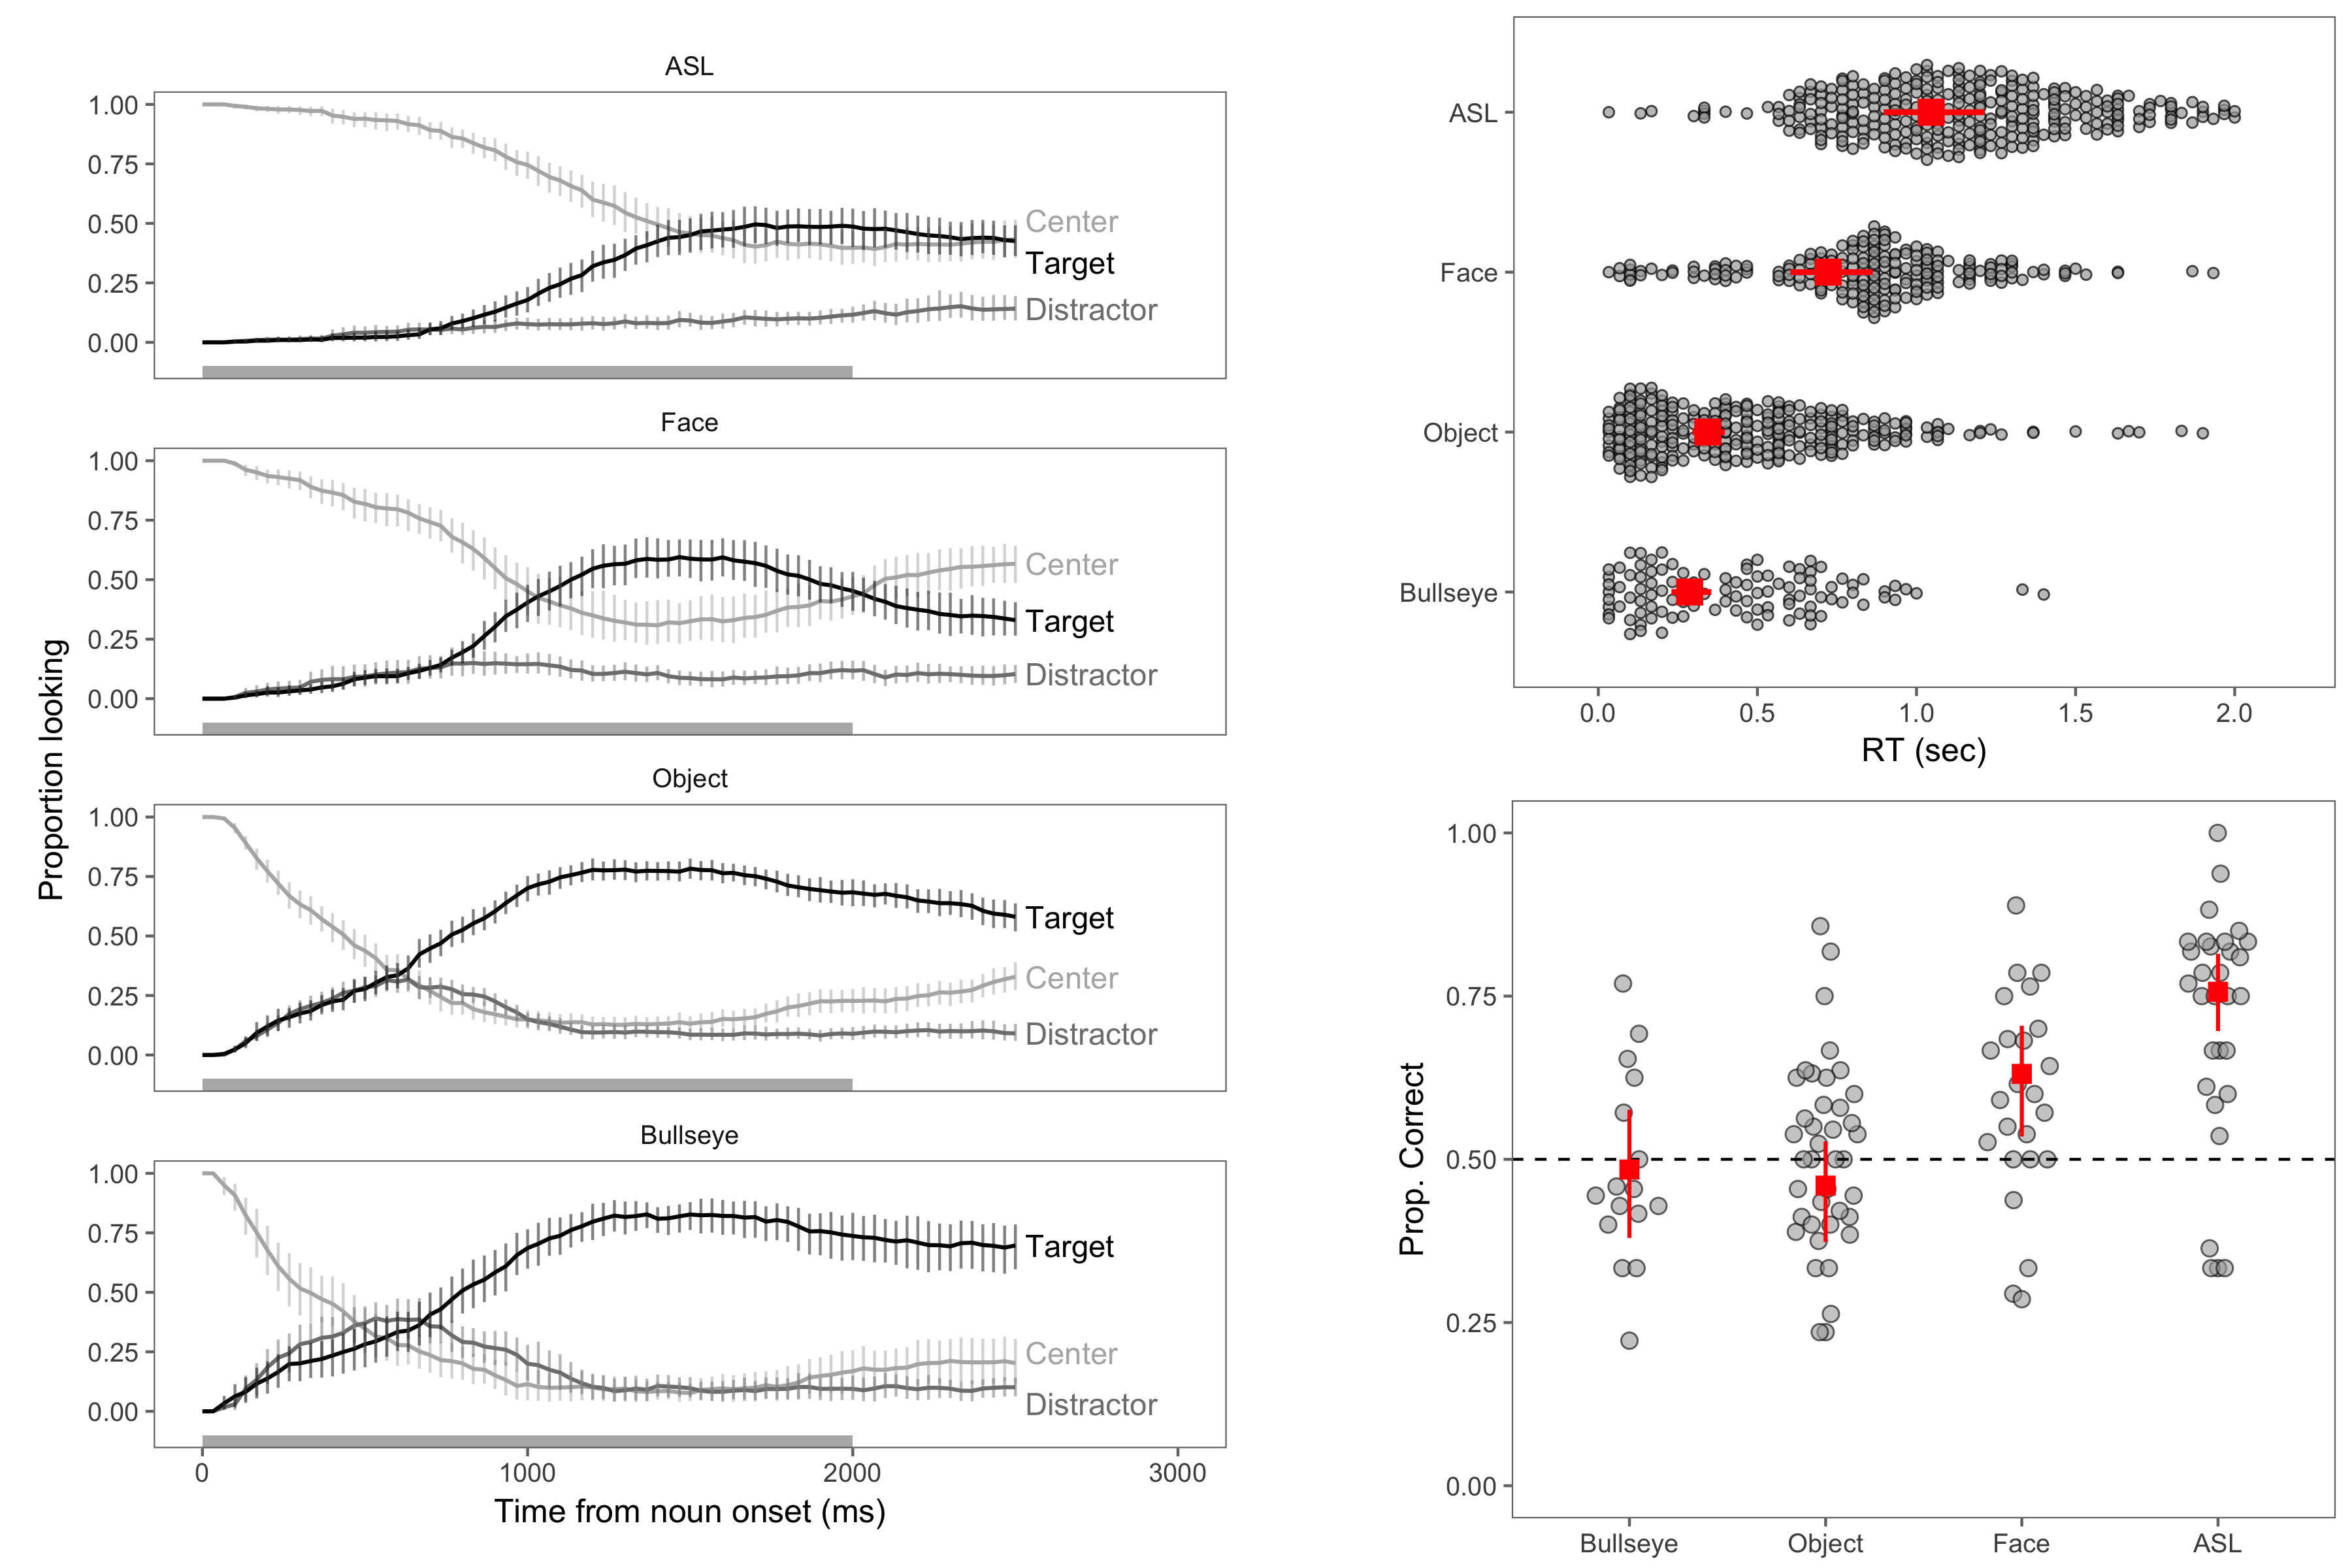
\includegraphics[width=0.9\linewidth]{/Users/kmacdonald/Documents/Projects/SPEED-ACC/paper/journal_submission/figures/figs_output//fig1_trio_behav} 

}

\caption{Timecourse looking, first shift Reaction Time (RT), and Accuracy results for children in Experiment 1. Panel A shows the overall looking to the center, target, and distracter stimulus for each context. Panel B shows the distribution of RTs for each participant. Each point represents a participant's average RT. Color represents the processing context. Panel C shows the same information but for first shift accuracy.}\label{fig:speed-acc-trio-plot}
\end{figure}

\hypertarget{behavioral-analyses}{%
\subsubsection{Behavioral analyses}\label{behavioral-analyses}}

\emph{Time course looking.} The first question of interest was how do
young ASL and English learners distribute attention across the three
fixation locations while processing language in real-time?Figure
~\ref{fig:speed-acc-trio-plot}A presents an overview of children's
looking to the center, target, and distracter images for each processing
context. This plot shows changes in the mean proportion of trials on
which participants fixated the signer, the target image, or the
distracter image at every 33-ms interval of the stimulus sentence. At
target-noun onset, children were looking at the center on all trials. As
the target noun unfolded, the mean proportion looking to the center
decreased rapidly as participants shifted their gaze to the target or
the distracter image. Proportion looking to the target increased sooner
and reached a higher asymptote, compared to proportion looking to the
distracter, for all four processing contexts.

After looking to the target image, participants tended to shift their
gaze back to the center, shown by the increase in proportion looking to
the center around two seconds after target-noun onset. There were
several qualitative differences in looking behavior across the different
center stimulus types. First, both ASL- and English-learners who
processed sentences from a video of speaker spent more time looking to
the center as indicated by the shallower slope on their center-looking
curves. Second, when the center stimulus was a static geometric object
(Bullseye) or a static familiar object (Object), spoken language
learners were more likely to look at the distracter image, especially
early in the time course of the target noun as indicated by the parallel
increase in target and distracter-looking curves in Figure
~\ref{fig:speed-acc-trio-plot}. In contrast, spoken language learners in
the Face context spent less time looking at the disracter, and
ASL-learners rarely looked to the distracter image at any point in the
trial. This pattern of behavior provides qualitative evidence that
children adpated their gaze depending on the nature of the visual world
and the modality of their language.

We tested differences in proportion looking to the center using a
nonparametric cluster-based permutation analysis, which accounts for the
issue of taking multiple comparisons across many time bins in the
timecourse (Maris \& Oostenveld, 2007). The center-looking curve for the
ASL learners was significantly different from all other conditions (all
p \textless{} .001). Within the spoken language groups, children's
looking to a speaker's face was different from looking to the Bullseye
and the Familar object (p \textless{} .001). Finally, the Object and
Bullseye center-looking curves were not different from one another, with
no significant differences at any point in the timecourse. Next, we ask
how these different processing contexts changed the timing and accuracy
of children's decisions to shift away from the center stimulus.

\emph{RT.} Figure ~\ref{fig:speed-acc-trio-plot}B shows the full RT data
distribution. To quantify differences across the groups, we fit a
Bayesian linear mixed-effects regression predicting first shift RT as a
function of center stimulus type, controlling for age, and including
user-defined contrasts to test specific comparisons of interest:
\texttt{Log(RT) $\sim$ center stimulus type + age +  (1 | subject) + (1 | item)}.
ASL learners generated slower RTs compared to all of the spoken English
samples (\(\beta\) = 0.60 sec, 95\% HDI {[}0.44 sec, 0.76 sec{]}).
Moreover, ASL learners' shifts were slower compared directly to children
processing spoken language in the Face condition (\(\beta\) = 0.32 sec,
95\% HDI {[}0.13 sec, 0.52 sec{]}). Finally, children in the Face
context shifted gaze slower compared to participants in the Object and
Bullseye contexts (\(\beta\) = 0.41 sec, 95\% HDI {[}0.29 sec, 0.55
sec{]}).

\emph{Accuracy.} Next, we compared the accuracy of first shifts across
the different tasks (Figure ~\ref{fig:speed-acc-trio-plot}C) by fitting
a mixed-effects logistic regression with the same specifications and
contrasts as the RT model. We found that (a) ASL learners were more
accurate compared to all of the spoken English samples (\(\beta\) =
0.23, 95\% HDI {[}0.17{]}, 0.29), (b) ASL learners were more accurate
when directly compared to participants in the Face task (\(\beta\) =
0.13, 95\% HDI {[}0.04, 0.23{]}), (c) children learning spoken language
were more accurate when processing language from dynamic video of a
person speaking compared to the Object and Bullseye tasks (\(\beta\) =
0.16, 95\% HDI {[}0.07, 0.24{]}), and (d) English-learners' first shifts
were no different from random responding in the Object (\(\beta\) =
-0.04, 95\% HDI {[}-0.13, 0.03{]}) and Bullseye (\(\beta\) = -0.02, 95\%
HDI {[}-0.12, 0.08{]}) contexts.

\hypertarget{model-based-analyses}{%
\subsubsection{Model-based analyses}\label{model-based-analyses}}

\begin{figure}[!t]

{\centering 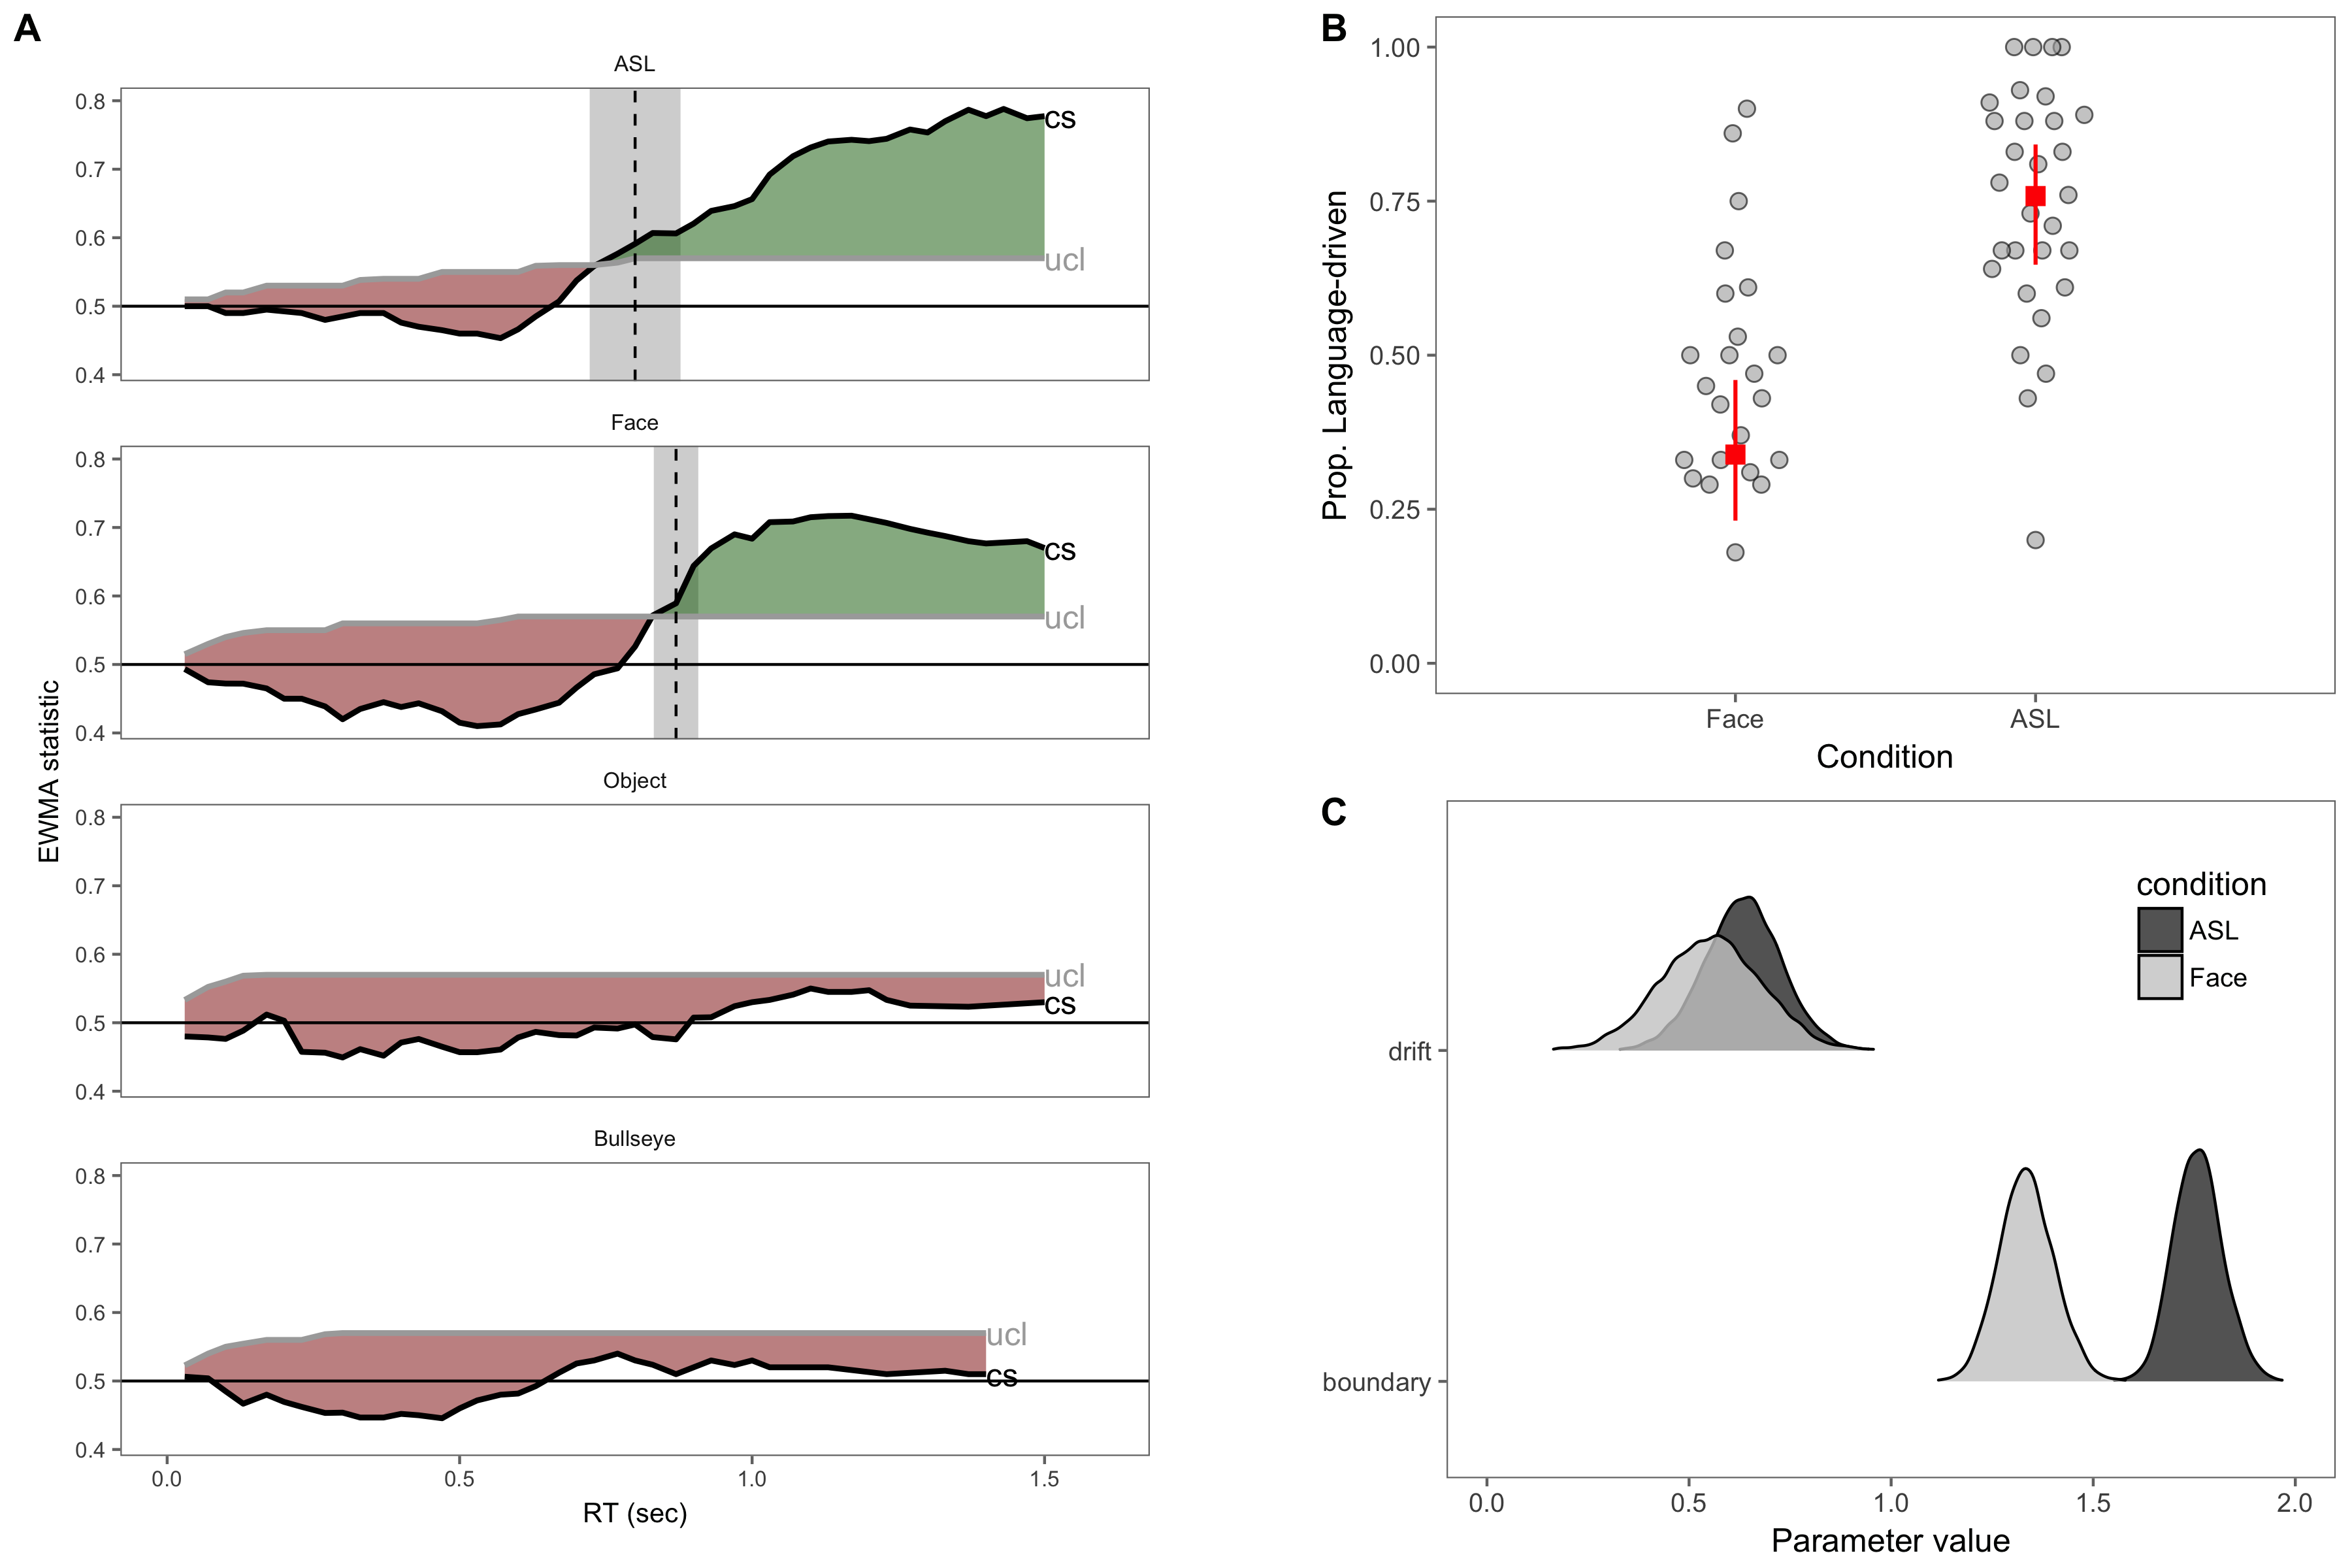
\includegraphics[width=0.9\linewidth]{/Users/kmacdonald/Documents/Projects/SPEED-ACC/paper/journal_submission/figures/figs_output//fig2_trio_models} 

}

\caption{Results for the model-based analyses in Experiment 1. Panel A shows a control chart representing the timecourse of the EWMA statistic. The black curve represents the evolution of the control statistic (CS) as a function of reaction time. The grey curve represents the upper control limit (UCL). The vertical dashed line is the median cutoff value (point when the control process shifts out of a guessing state). The grey shaded area represents the 95\% Confidence Interval around the estimate of the median cutoff point, and the shaded ribbons represent the proportion of responses that were categorized as guesses (red) and language-driven (green). Panel B shows a summary of the proportion of shifts that were categorized as language-driven for the Face and ASL processing contexts. Panel C shows the point estimate and 95\% Highest Density Intervals for the boundary and drift rate parameters for the Face and ASL contexts.}\label{fig:trio-model-plot}
\end{figure}

\emph{EWMA.} Our third question of interest was how the tendency to
generate random vs.~language-driven (i.e, accurate) gaze shifts evolved
as a function of reaction time across the different processing contexts.
Figure ~\ref{fig:trio-model-plot}A shows changes in the control
statistic (CS, weighted moving average) and the upper control limit
(UCL, upper threshold on guessing) as a function of RT. Each CS starts
at chance performance and below the UCL. In the ASL and Face tasks, the
CS value begins to increase with RTs around 0.7 seconds after noun onset
and eventually crosses the UCL, indicating that responses \textgreater{}
0.7 sec were on average above chance levels. In contrast, the CS in the
Object and Bullseye tasks never crossed the UCL, indicating that
children's shifts were equally likely to land on the target or the
distracter, regardless of when they were initiated. This result suggests
that first shifts measured in the Bullseye/Object tasks were
qualitatively different behaviors than those in the ASL and Face
contexts. That is, these shifts are likely the result of a different
generative process such as gathering more information about the
referents in the visual world.

Next, we compared the EWMA model fits for participants in the ASL and
Face processing contexts since these groups showed evidence of
language-driven responding. We found that ASL learners generated fewer
shifts when the CS was below the UCL compared to children learning
spoken language (\(\beta\) = 0.14, 95\% HDI {[}0.08, 0.23{]}). This
result indicates that ASL-learners were more likely to have gathered
sufficient information about the linguistic signal prior to shifting
gaze away from the language source. We found some evidence that ASL
learners started producing language-driven shifts earlier in the RT
distribution as indicated by the point at which the CS crossed the UCL
(\(\beta\) = 0.22 sec, 95\% HDI {[}0.05 sec, 0.39 sec{]}), indicating
that these children were less likely to generate early, random gaze
shifts away from the signer.

\emph{HDDM.} We fit a hierarchical Drift Diffusion Model using only the
gaze shifts categorized as language-driven by the EWMA. This allowed us
to ask what underlying decision processes are likely to account for the
measured differences in First Shift Accuracy and RT.\footnote{We chose
  not to interpret the HDDM fits for the Bullseye or Face tasks since
  there was no suggestion of any non-guessing signal from the EWMA
  analysis.} ASL learners had a higher estimate for the boundary
separation parameter compared to children processing spoken English from
a speaker (ASL boundary = 1.76, 95\% HDI {[}1.65, 1.88{]}; Face boundary
= 1.34, 95\% HDI {[}1.21, 1.47{]}), with no overlap in the credible
values (see Figure ~\ref{fig:trio-model-plot}). This suggests that ASL
learners' higher accuracy was driven by accumulating more evidence about
the linguistic signal before generating an eye movement. We found high
overlap for estimates of the drift rate parameter, indicating that both
groups processed the linguistic information with similar efficiency (ASL
drift = 0.63, 95\% HDI {[}0.44, 0.82{]}; Face drift = 0.55, 95\% HDI
{[}0.30, 0.80{]}).

\emph{Results summary.} Taken together, the behavioral and model-based
analyses provide converging support that ASL learners were sensitive to
the value of delaying eye movements away from the language source.
Compared to spoken language learners, ASL learners prioritized accuracy
over speed (HDDM), produced fewer nonlanguage-driven shifts away from
the center stimulus (EWMA), and were more accurate with these gaze
shifts (behavioral). Importantly, we did not see evidence in the HDDM
model fits that these accuracy differences could be explained by
differential efficiency in processing the linguistic information.
Instead, the pattern of results suggests that ASL learners increased
their decision threshold for generating a gaze shift away from a signer
to a named object.

We hypothesized that prioritizing accuracy of gaze shifts above speed of
responding when processing a visual-manual language is an adaptive
response. That is, to map referential language to the visual world in
ASL involves competition for visual attention. When ASL learners choose
to shift their gaze away from a signer, they are leaving an area that
provides a great deal of useful information. Moreover, unlike children
learning spoken languages, ASL learners cannot gather more of the
linguistic signal if their gaze is directed away from a signer. Thus, it
seems reasonable that ASL learners would adapt the timing of their gaze
shifts to gather additional information that increases certainty in
comprehension before seeking a named object.

It is important to point out that these findings were based on
exploratory analyses, and our information seeking account was developed
to explain this pattern of results. There are, however, several,
potentially important differences between the stimuli, apparatus, and
populations that limit the strength of our interpretation and the
generality of our account. Moreover, we cannot interpret these any
causal effects because we are comparing children who are learning
different languages. Thus, we designed Experiments 2 and 3 to address
these concerns and set out to perform well-controlled, experimental
tests of our information seeking account of eye movements in grounded,
social language comprehension.

\hypertarget{experiment-2}{%
\section{Experiment 2}\label{experiment-2}}

In Experiment 2, we aimed to replicate a key finding from Experiment 1:
that increasing the competition between fixating on a language source
and the nonlinguistic visual world reduces nonlanguage-driven eye
movements. Moreover, we conducted a confirmatory test of our hypothesis
that controlled for the population differences present in Experiment 1.
We tested a sample of English-speaking adults using a
within-participants manipulation of the language-relevance of the center
stimulus. We used the Face and Bullseye stimulus sets from Experiment 1
and added two new conditions: (1) Text, where the verbal language
information was accompanied by a word-by-word display of printed text
(see Figure ~\ref{fig:trio-stim}), and Text-no-audio, where the spoken
language stimulus was removed. We chose text processing since, like sign
language comprehension, information relevant to the linguistic signal is
concentrated in one location in the visual scene.

Our key behavioral prediction is that processing serially-presented text
will shift the value of allocating fixations to the center stimulus as
the linguistic information unfolds in time. This shift in information
value should result in listeners allocating more fixations to the center
stimulus and fewer to the objects in the visual scene. This behavioral
pattern should be indexed by proportion guessing and cutoff point
parameters of the EWMA model. We did not have strong predictions for
First Shift Accuracy, Reaction Time, or the HDDM parameter fits since
the goal of the text manipulation was to modulate participants'
strategic allocation of visual attention and not the accuracy/efficiency
of information processing.

\hypertarget{methods-1}{%
\subsection{Methods}\label{methods-1}}

\hypertarget{participants-1}{%
\subsubsection{Participants}\label{participants-1}}

24 Stanford undergraduates participated (5 male) for course credit. All
participants were monolingual, native English speakers and had normal
vision.

\hypertarget{stimuli-1}{%
\subsubsection{Stimuli}\label{stimuli-1}}

Audio and visual stimuli were identical to the Face and Bullseye tasks
in Experiment 1. We included a new center fixation stimulus type:
printed text. The text was displayed in a white font on a black
background and was programmed such that only a single word appeared on
the screen, with each word appearing for the same duration as the
corresponding word in the spoken language stimuli.

\hypertarget{design-and-procedure-1}{%
\subsubsection{Design and procedure}\label{design-and-procedure-1}}

The design was nearly identical to Experiment 1, with the exception of a
change to a within-subjects manipulation where each participant
completed all four tasks (Bullseye, Face, Text, and Text-no-audio). In
the Text condition, spoken language accompanied the printed text. In the
Text-no-audio condition, the spoken language stimulus was removed.
Participants saw a total of 128 trials while their gaze was tracked
using an SMI RED corneal-reflection eye-tracker mounted on an LCD
monitor, sampling at 30 Hz. The eye-tracker was first calibrated for
each participant using a 6-point calibration.

\hypertarget{results-and-discussion-1}{%
\subsection{Results and Discussion}\label{results-and-discussion-1}}

\begin{figure}[!t]

{\centering 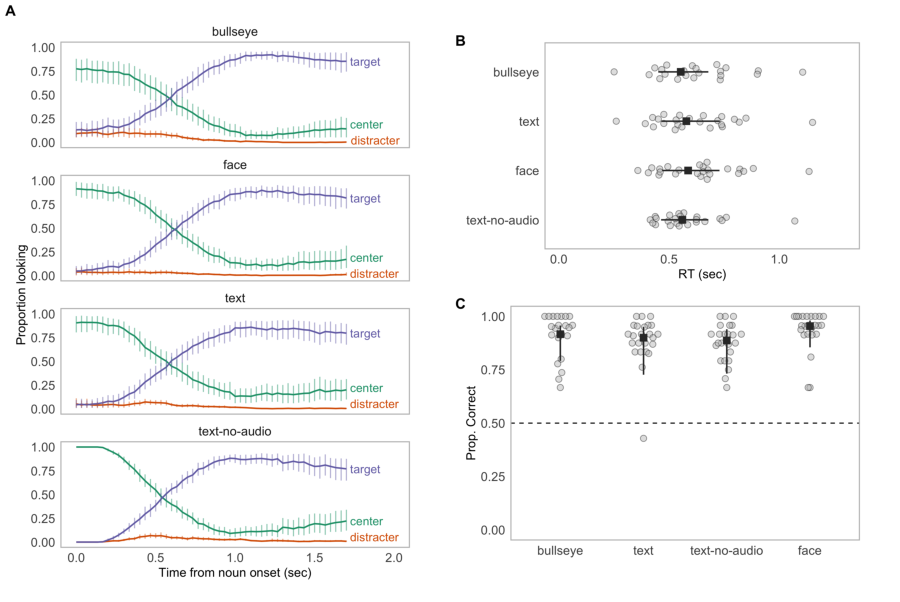
\includegraphics[width=0.9\linewidth]{figs/text-plot-1} 

}

\caption{Results for the model-based analyses in Experiment 2. All plotting conventions are the same as in Figure 2.}\label{fig:text-plot}
\end{figure}

\hypertarget{behavioral-analyses-1}{%
\subsubsection{Behavioral analyses}\label{behavioral-analyses-1}}

\emph{Timecourse looking.} Panel A of Figure ~\ref{fig:text-plot}
presents an overview of adults's looking to the center stimulus, target,
and distracter images for each center stimulus type. Similar to
children's looking behavior in Experiment 1, at target-noun onset the
majority of adults were looking at the center. As the target noun
unfolded, the mean proportion looking to the center decreased rapidly as
participants shifted their gaze to the objects. Proportion looking to
the target increased sooner and reached a higher asymptote compared to
proportion looking to the distracter for all four processing contexts.

After looking to the target image, adults did not tend to shift their
gaze back to the center as shown by the relatively flat proportion
looking to center curves at approximately one second after target-noun
onset. The primary qualitative difference in adult's looking behavior
across the different center stimulus types was a higher tendency to be
looking at the center stimulus in the Face and Text conditions relative
to the Bullseye condition. This was especially true for the
Text-no-audio condition where adults were looking to the center at
target-noun onset on 100\% of the trials. A cluster-based permutation
analysis confrimed that there were significant differences in looking to
the center stimulus between the Text-no-audio and the Bullseye, Face,
and Text conditions (all ps \textless{} .001). This pattern of behavior
provides preliminary evidence that making all of the linguistic
information visual changed adults' looking behavior early in the
timecourse of the target noun.

\emph{RT.} Visual inspection of Figure ~\ref{fig:text-plot}C suggests
that mean response times of first shifts were similar across the four
center stimulus conditions (\(M_{bull}\) = 0.55 sec, \(M_{face}\) = 0.59
sec, \(M_{text}\) = 0.58 sec, \(M_{textNoaudio}\) = 0.56 sec). We fit a
linear mixed-effects regression with the same specification as in
Experiment 1, but we added by-subject intercepts and slopes for each
center stimulus type to account for our within-subjects manipulation. We
did not see evidence that mean RTs were different across the conditions,
with the null value of zero condition differences falling within the
95\% HDIs for each contrast of interest (see table TODO in the appendix
for the full model output).

\emph{Accuracy.} Next, we modeled accuracy using a mixed-effects
logistic regression with the same specifications (see Panel B of Figure
~\ref{fig:text-plot}). We found that adults' first shifts were highly
accurate and performed similarly across the four conditions
(\(M_{bullseye}\) = 0.92, \(M_{face}\) = 0.95, \(M_{text}\) = 0.90,
\(M_{textNoAudio}\) = 0.89). In contrast to the children in Experiment
1, adults' responses were above chance level even in the Bullseye
condition when the center stimulus was not salient or informative (see
table TODO in the appendix for the full ouput of the accuracy model).

Adults' accurate first shifts suggests an interesting developmental
difference in the construal of the center stimulus in our task. This is
speculative, but it seems plausible that adults thought the Bullseye was
designed to be a valid starting point for fixating gaze while the
sentence unfolded (i.e., someone put this here for a reason). As a
result, if adults maintained their fixation on the center stimulus for
enough time to gather sufficient linguistic singal, then they were
highly accurate across all four processing conditions, which is
reasonable since these were highly familiar words presented in
child-directed speech.

Visual inspection of the timecourse looking curves, however, suggests
that the effect of the text manipulations occurred earlier in timecourse
of decisions about visual fixation. That is, in the first 300 ms after
the start of the target word adults in the Bullseye, Face, and Text
conditions were already allocating fixations away from the center
stimulus and to the objects. In contrast, in the Text-No-Audio
condition, where adults did not have access to linguistic information
via the auditory channel, all of the fixations were focused on the
center stimulus location. Next, we use our model-based analyses to
quantify these differences in adults' decisions about where to fixate as
a function of time.

\hypertarget{model-based-analyses-1}{%
\subsubsection{Model-based analyses}\label{model-based-analyses-1}}

\begin{figure}[!t]

{\centering 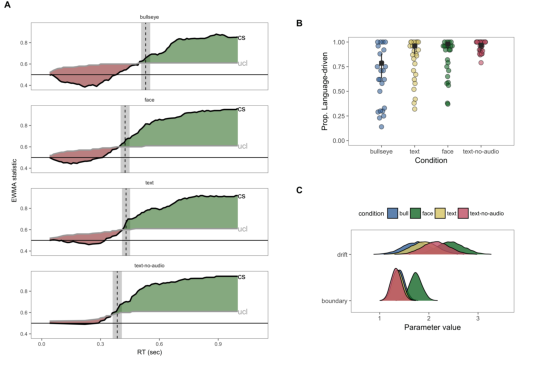
\includegraphics[width=0.9\linewidth]{figs/text-model-plots-1} 

}

\caption{Results for the model-based analyses of Experiment 2. All plotting conventions are the same as Figure 3.}\label{fig:text-model-plots}
\end{figure}

\emph{EWMA.} For all four conditions, the control statistic crossed the
upper control limit (Figure ~\ref{fig:text-model-plots}A), suggesting
that adults' shifts were reliably driven by linguistic information at
some point in the RT distribution. There was a graded effect of
condition on the cutoff point (see the horizontal shift in the vertical
dashed lines in Panel A). That is, the CS crossed the UCL earliest in
the Text-no-audio condition (\(M_{text-no-audio}\) = 0.39, 95\% HDI
{[}0.37, 0.41{]}), followed by the Text (\(M_{text}\) = 0.44, 95\% HDI
{[}0.42, 0.46{]}) and Face (\(M_{face}\) = 0.45, 95\% HDI {[}0.43,
0.47{]}) conditions, and finally the Bullseye condition
(\(M_{bullseye}\) = 0.54, 95\% HDI {[}0.52, 0.56{]}).\footnote{See Table
  TODO in the appendix for the relevant statistics for the pairwise
  comparisons of interest.}

We also found a graded difference in the proportion of shifts that
occurred when the control statistic was below the upper control limit
(\(M_{bullseye}\) = 0.78, \(M_{text}\) = 0.86, \(M_{text-no-audio}\) =
0.89, \(M_{face}\) = 0.93). Adults generated fewer language-driveneye
movements in the Bullseye condition as compared to the other contexts
(\(\beta\) = -0.12, 95\% HDI {[}-0.26, -0.01{]}), and the highest
proportion of language-driven shifts in the Text-no-audio context
(\(\beta\) = 0.04, 95\% HDI {[}-0.02, 0.08{]}). These results provide
evidence for our key prediction: that increasing the value of fixating
on the center stimulus for accessing linguistic information reduced
early gaze shifts to the rest of the visual world. This shift in gaze
dynamics, in turn, resulted in adults generating fewer eye movements
away from the center stimulus early in the timecourse of the target
noun, leading to a higher proportion of language-driven shifts.

\emph{HDDM.} Using the classifications generated by the EWMA, we fit an
HDDM to the language-driven shifts with the same specifications as in
Experiment 1. There was high overlap of the posterior distributions for
the drift rate parameters (see panel C of Figure 5), suggesting that
participants gathered the linguistic information with similar
efficiency. We also found high overlap in the distribution of boundary
separation estimates for the Bullseye, Text, and Text-no-audio
conditions. We saw some evidence for a higher boundary separation in the
Face condition compared to the other three center stimulus types (Face
boundary = 1.73, HDI = {[}1.49, 1.98{]}; Bullseye boundary = 1.40, HDI =
{[}1.19, 1.62{]}; Text boundary = 1.37, HDI = {[}1.16, 1.58{]};
Text-no-audio boundary = 1.34, HDI = {[}1.14, 1.55{]}), indicating that
adults' were accumulating more information before generating before
shifting gaze away from a speaker's face. Note that the higher boundary
separation and drift rate parameters in this context differs from the
results of the standard Accuracy and Reaction Time analyses, which found
similar patterns of performance. This likely occurs because the HDDM
estimates parameters by integrating information from RT distributions
for both correct and incorrect responses.

\emph{Results summary.} These results suggest that when adults were
processing serially-presented text, they were less likely to generate
nonlangauge-driven shifts to the objects (EWMA results) but their
efficiency of processing the linguistic signal itself did not change
(Accuracy, RT, and HDDM results). Interestingly, we found a graded
difference in the EWMA results between the Text and Text-no-audio
conditions, with the lowest proportion of early, nonlanguage-driven
shifts occurring when adults' processed text without accompanied verbal
language. This behavior seems reasonable; if the adults could rely on
the auditory channel to gather the linguistic information, then the
value of fixating on the text display decreases. In contrast to the
children in Experiment 1, adults were highly accurate in the Bullseye
condition, perhaps because they construed the Bullseye as a center
fixation that they \emph{should} fixate, or perhaps they had better
encoded the location/identity of the two referents prior to the start of
the target sentence.

The results of Experiment 2, however, are limited in several ways.
First, the text manipulation did not result in a clear difference in
first shift accuracy or reaction time. We think this might be caused by
ceiling effects in our paradigm since adults are so highly practiced at
recognizing the familiar nouns used in the task. Second, while
serially-presented text shares some features with processing a
visual-manual language like ASL, it is nonetheless a very different
cognitive task. Moreover, text is typically scanned by a reader and not
presented word-by-word. Thus, we want to be careful to not making any
claims about absolute differences in how rapidly or accurately text is
processed relative to spoken language. Finally, and most importantly for
our theoretical account, the text paradigm is not suitable for our
target age range: young children acquiring their first language. Thus,
we designed Experiment 3 to be a well-controlled test of our information
seeking account that (1) used a manipulation within the domain of spoken
language comprehension and (2) could be used with both adults and
children.

\hypertarget{experiment-3}{%
\section{Experiment 3}\label{experiment-3}}

In Experiment 3, we measured adults and children's eye movements during
a real-time language comprehension task where participants processed
familiar sentences (e.g., \enquote{Where's the ball?}) while looking at
a simplified visual world with three fixation targets. Using a
within-participants design, we manipulated the signal-to-noise ratio of
the auditory signal by convolving the acoustic input with brown noise
(random noise with greater energy at lower frequencies).

We predicted that processing speech in a noisy context would make
participants less likely to shift before collecting sufficient
information.\footnote{See \url{https://osf.io/g8h9r/} for a
  pre-registration of the analysis plan.} This delay, in turn, would
lead to a lower proportion of shifts flagged as random/exploratory in
the EWMA analysis, and a pattern of HDDM results indicating a
prioritization of accuracy over and above speed of responding (see the
Analysis Plan section below for more details on the models). We also
predicted a developmental difference: that children would produce a
higher proportion of random shifts and accumulate information less
efficiently compared to adults, and a developmental parallel: that
children would show the same pattern of adapting gaze patterns to gather
more visual information in the noisy processing context.

\hypertarget{methods-2}{%
\subsection{Methods}\label{methods-2}}

\hypertarget{participants-2}{%
\subsubsection{Participants}\label{participants-2}}

Participants were native, monolingual English-learning children (\(n=\)
39; 22 F) and adults (\(n=\) 31; 22 F). All participants had no reported
history of developmental or language delay and normal vision. 14
participants (11 children, 3 adults) were run but not included in the
analysis because either the eye tracker falied to calibrate (2 children,
3 adults) or the participant did not complete the task (9 children).

\hypertarget{stimuli-2}{%
\subsubsection{Stimuli}\label{stimuli-2}}

\emph{Linguistic stimuli.} The video/audio stimuli were recorded in a
sound-proof room and featured two female speakers who used natural
child-directed speech and said one of two phrases: \enquote{Hey! Can you
find the (target word)} or "Look! Where's the (target word). The target
words were: ball, bunny, boat, bottle, cookie, juice, chicken, and shoe.
The target words varied in length (shortest = 411.68 ms, longest =
779.62 ms) with an average length of 586.71 ms.

\emph{Noise manipulation}. To create the stimuli in the noise condition,
we convolved each recording with Brown noise using the Audacity audio
editor. The average signal-to-noise ratio (values greater than 0 dB
indicate more signal than noise) in the noise condition was 2.87 dB
compared to the clear condition, which was 35.05 dB.

\emph{Visual stimuli.} The image set consisted of colorful digitized
pictures of objects presented in fixed pairs with no phonological
overlap between the target and the distracter image (cookie-bottle,
boat-juice, bunny-chicken, shoe-ball). The side of the target picture
was counterbalanced across trials.

\hypertarget{design-and-procedure-2}{%
\subsubsection{Design and procedure}\label{design-and-procedure-2}}

Participants viewed the task on a screen while their gaze was tracked
using an SMI RED corneal-reflection eye-tracker mounted on an LCD
monitor, sampling at 30 Hz. The eye-tracker was first calibrated for
each participant using a 6-point calibration. On each trial,
participants saw two images of familiar objects on the screen for two
seconds before the center stimulus appeared. Next, they processed the
target sentence -- which consisted of a carrier phrase, a target noun,
and a question -- followed by two seconds without language to allow for
a response. Child participants saw 32 trials (16 noise trials; 16 clear
trials) with several filler trials interspersed to maintain interest.
Adult participants saw 64 trials (32 noise; 32 clear). The noise
manipulation was presented in a blocked design with the order of block
counterbalanced across participants.

\hypertarget{results-and-discussion-2}{%
\subsection{Results and discussion}\label{results-and-discussion-2}}

\hypertarget{behavioral-analyses-2}{%
\subsubsection{Behavioral analyses:}\label{behavioral-analyses-2}}

\begin{figure}[!t]

{\centering 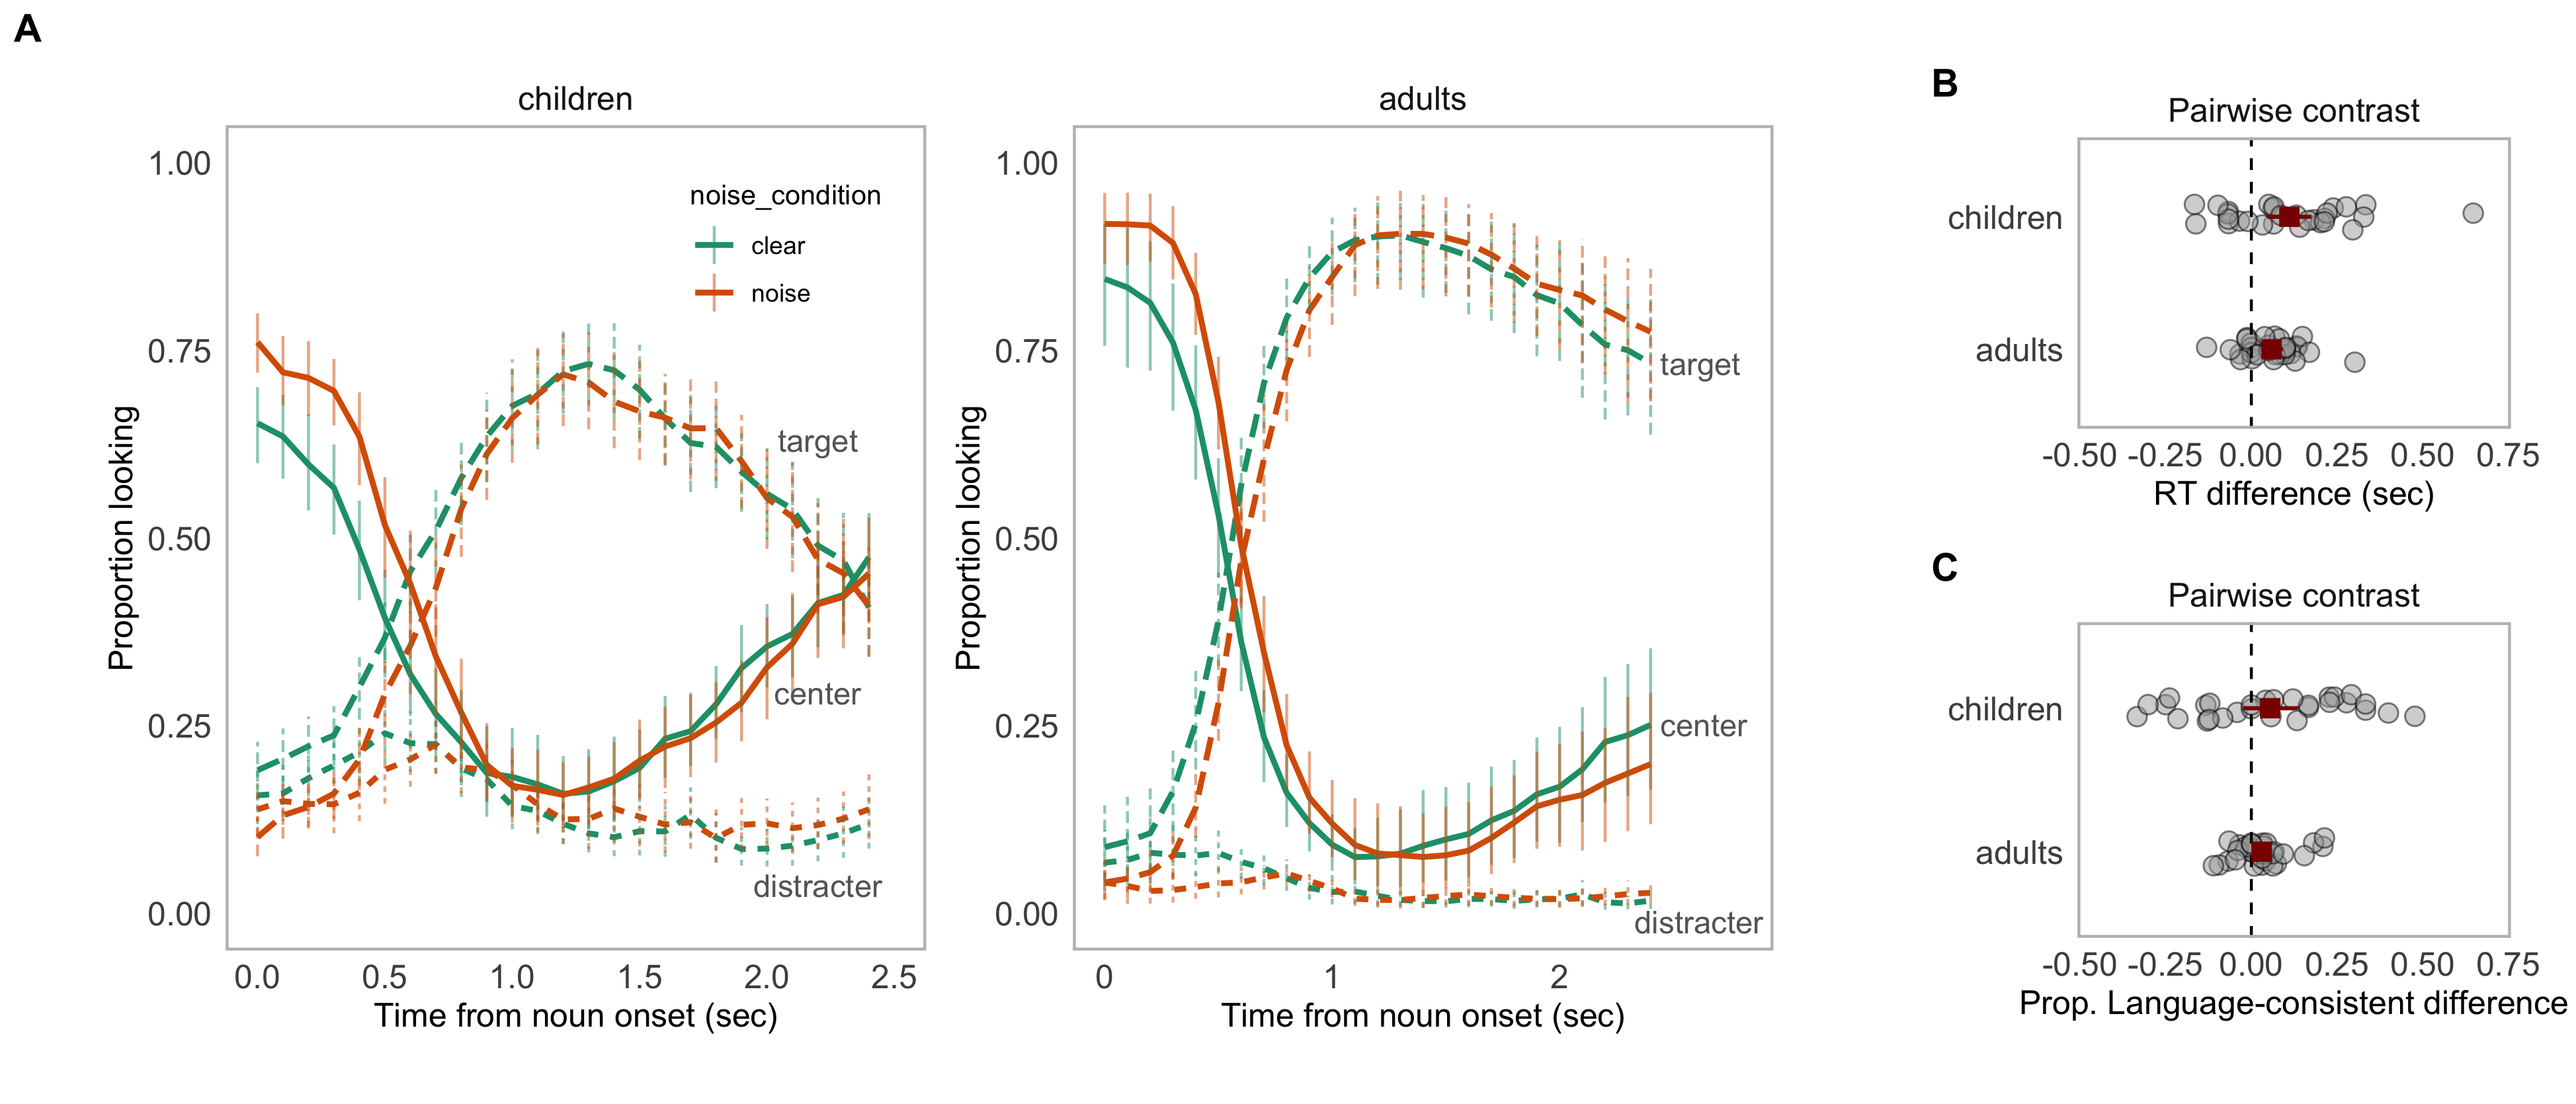
\includegraphics[width=0.9\linewidth]{/Users/kmacdonald/Documents/Projects/SPEED-ACC/paper/journal_submission/figures/figs_output//fig5_noise_behav} 

}

\caption{Behavioral results for children and adults in Experiment 3. Panel A shows the overall looking to the center, target, and distracter stimulus for each processing condition and age group. Panel B shows the distribution of RTs for each participant and the pairwise contrast between the noise and clear conditions. The square point represents the mean value for each mesure. The vertical dashed line represents the null model of zero condition difference. The width each point represents the 95\% HDI. Panel C shows the same information but for first shift accuracy.}\label{fig:noise-acc-rt-plot}
\end{figure}

\emph{Timecourse looking.} Figure ~\ref{fig:noise-acc-rt-plot}A presents
an overview of looking to the speaker, target, and distracter images for
the noisy and clear processing contexts from the start of the target
noun. Similar to the results in Experiment 1 and 2, participants tended
to fixate on the speaker at target-noun onset. As the target noun
unfolded, the mean proportion looking to the center decreased rapidly as
participants shifted their gaze to the objects. Proportion looking to
the target increased sooner and reached a higher asymptote compared to
proportion looking to the distracter for all four processing contexts.
After looking to the target image, participants tended to shift their
gaze back to the speaker as shown by the increase in center looking
curve around 1 second.

There are several developmental differences to highlight. First,
children tended to look more to the objects at noun onset, as indicated
by the lower intercept of children's center-looking curves. Second,
children's target looking curves reached a lower asymptote as compared
to adults and they spent relatively more time fixating on the distracter
image, whereas adults rarely looked at the unnamed object after 0.5
seconds in the timecourse of the trial. And third, children showed a
stronger tendency to shift back to the speaker after looking to the
named object.

Visual inspection of the center looking curve suggests a key conditon
difference in looking behavior for the noisy processing context. That
is, both children and adult's spent more time fixating on the speaker
when the auditory signal was less reliable as indicated by the shift to
the right in the center-looking curves for the noisy context. A
cluster-based permutation test confirmed that there was evidence of a
significant difference in looking to the speaker between the Noisy and
Clear conditions (ps \textless{} .05). This pattern of behavior provides
preliminary evidence that reducing the quality of the auditory signal
increased looking to the speaker early in the timecourse of the target
noun.

\emph{RT.} Figure ~\ref{fig:noise_acc_rt_noise_plot}A shows the full
distribution of the estimated RT differences between each participants'
performance in the noise and clear contexts. Both children and adults
were slower to identify the target in the noise condition (Children
\(M_{noise}\) = 500.19 sec; Adult \(M_{noise}\) = 595.23 sec), as
compared to the clear condition (Children \(M_{clear}\) = 455.72 sec
Adult \(M_{clear}\) = 542.45 sec). RTs in the noise condition were 48.82
seconds slower on average, with a 95\% HDI ranging from 3.72 sec to
96.26 ms, and not including the null value of zero condition difference.
Older children responded faster than younger children (\(M_{age}\) =
-0.44, {[}-0.74, -0.16{]}), with little evidence for an interaction
between age and condition.

\emph{Accuracy.} Next, we modeled adults and children's first shift
accuracy using a mixed-effects logistic regression with the same
specifications (Figure ~\ref{fig:noise_acc_rt_noise_plot}B). Both groups
were more accurate than a model of random responding (null value of
\(0.5\) falling well outside the lower bound of the 95\% HDI for all
group means). Adults were more accurate (\(M_{adults} =\) 90\%) than
children (\(M_{children} =\) 61\%). The key result is that both groups
showed evidence of higher accuracy in the noise condition: children
(\(M_{noise}\) = 67\%; \(M_{clear}\) = 61\%) and adults (\(M_{noise}\) =
92\%; \(M_{clear}\) = 90\%). Accuracy in the noise condition was on
average 4\% higher, with a 95\% HDI from -1\% to 12\%. Note that the
null value of zero difference falls at the very edge of the HDI. But
95\% of the credible values are greater than zero, providing evidence
for higher accuracy in the noise condition. Within the child sample,
there was no evidence of a main effect of age or an interaction between
age and noise condition.

\hypertarget{model-based-analyses-2}{%
\subsubsection{Model-based analyses:}\label{model-based-analyses-2}}

\begin{figure}[!t]

{\centering 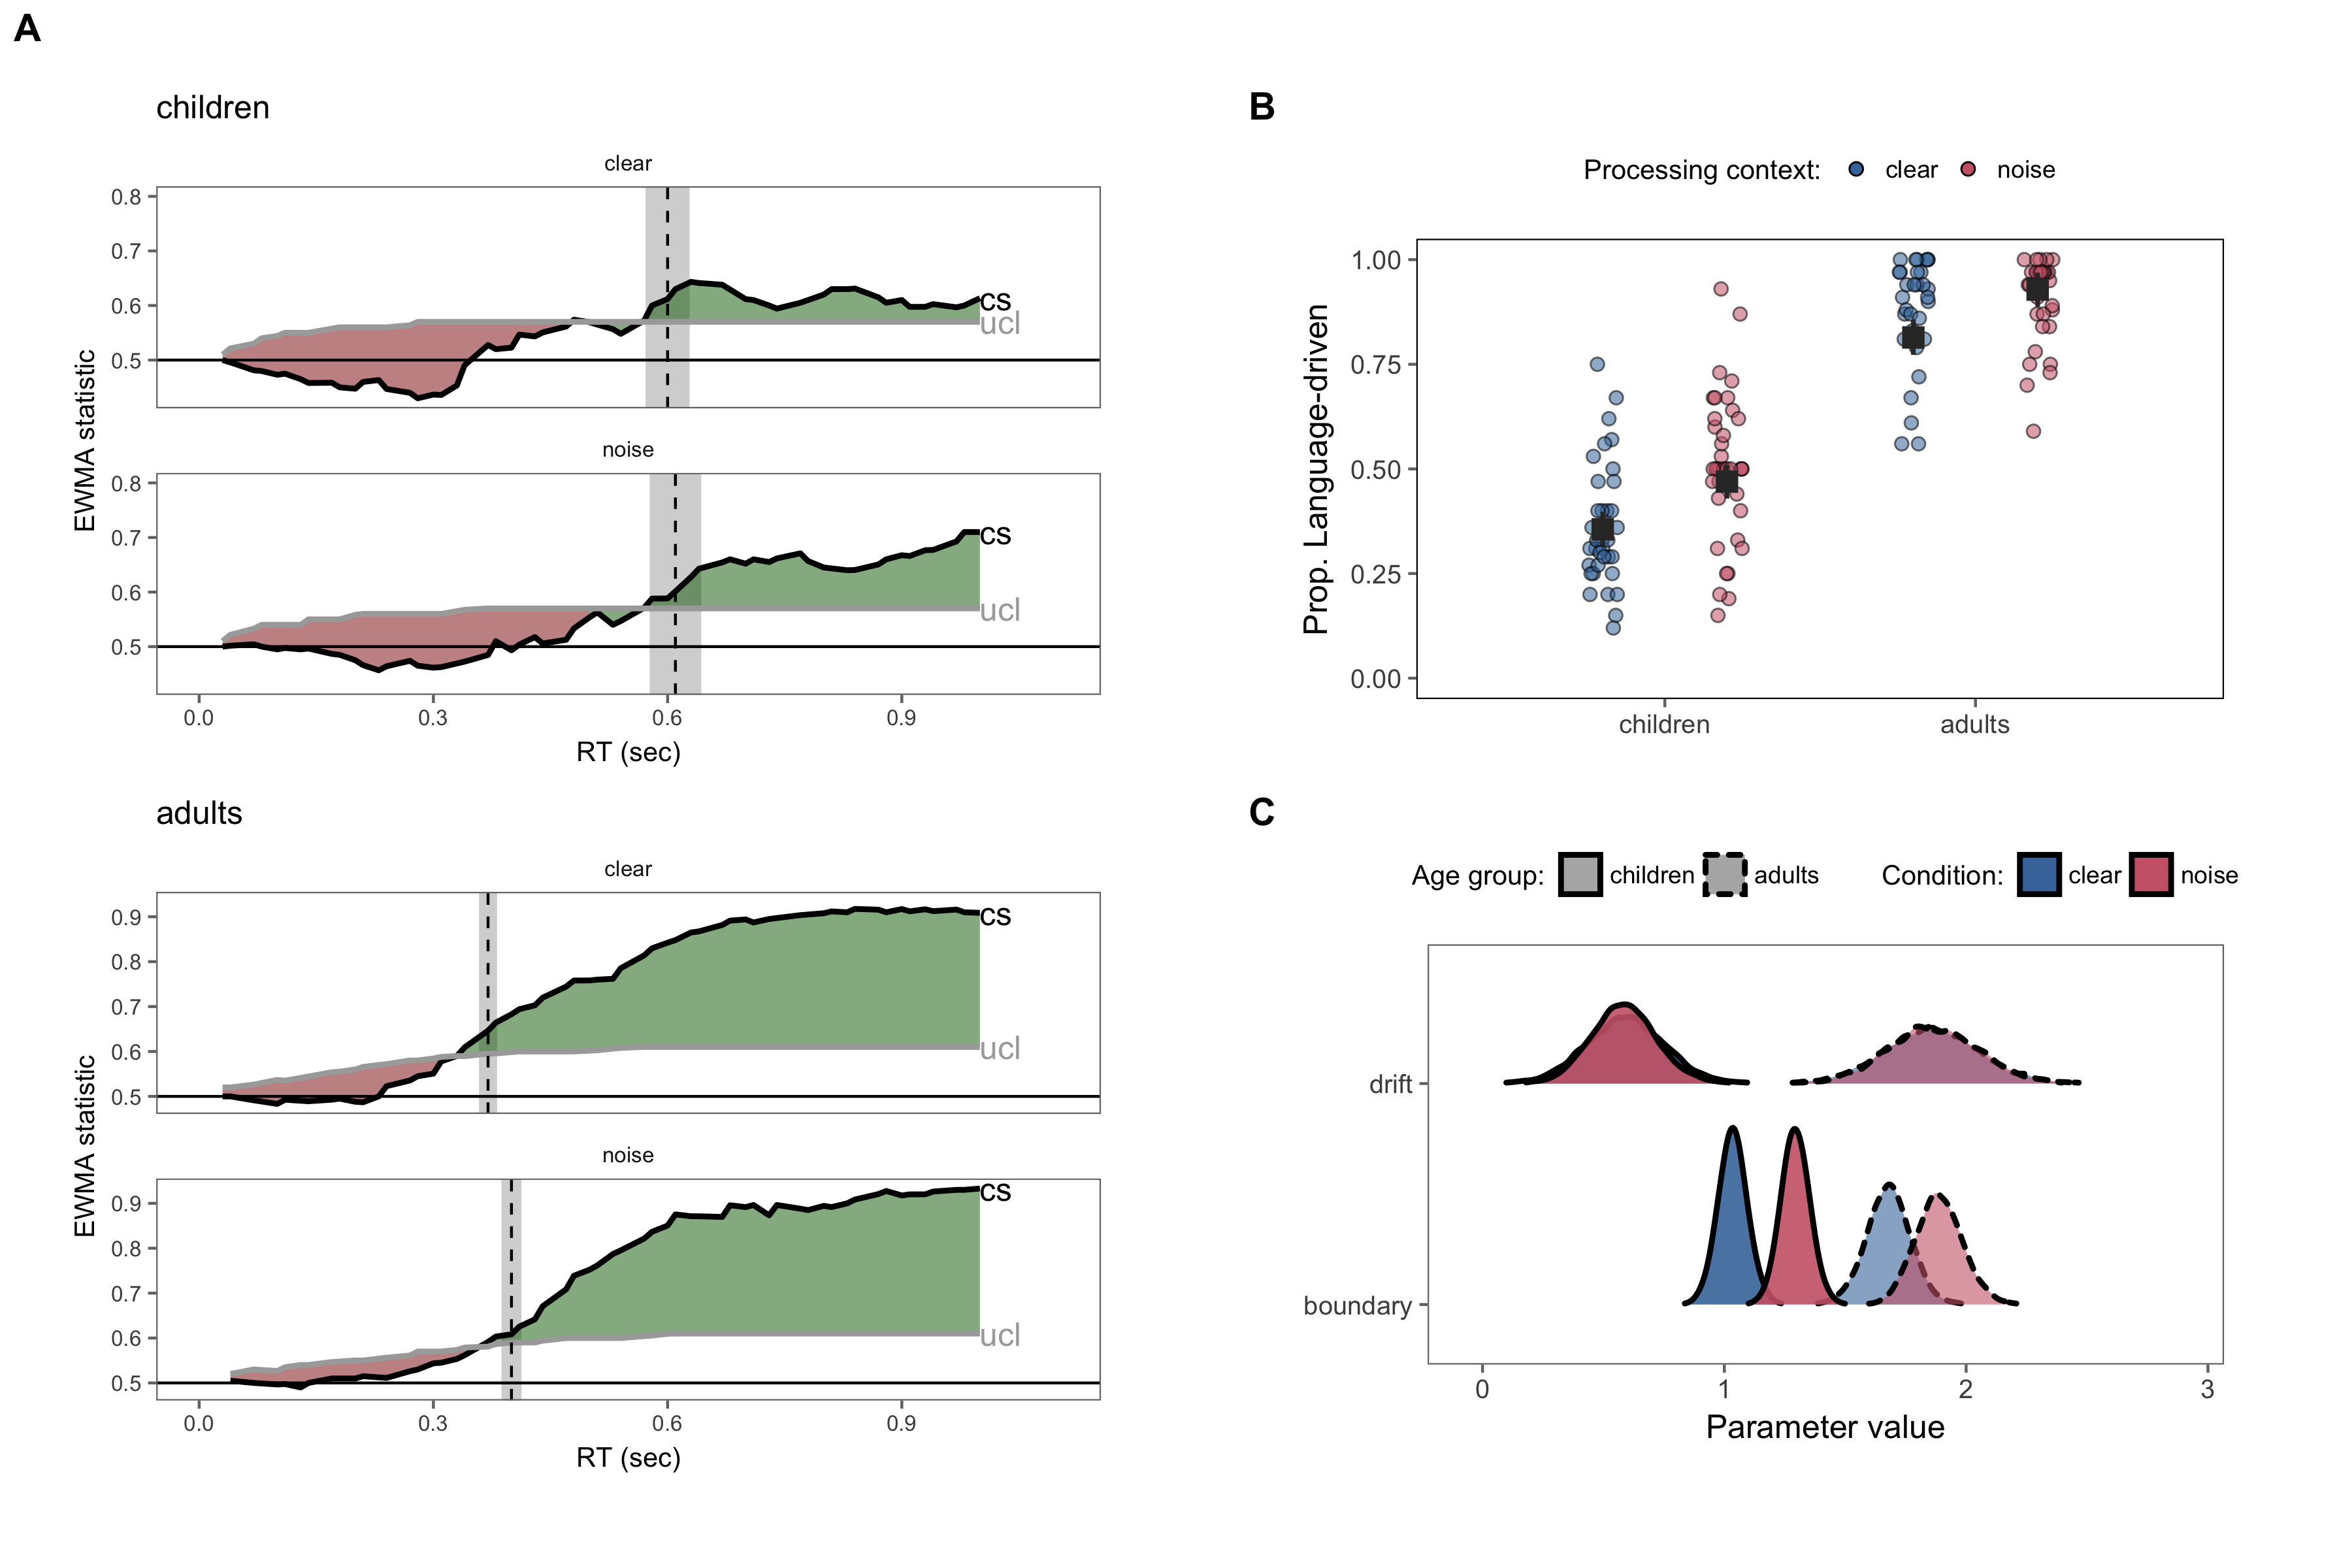
\includegraphics[width=0.9\linewidth]{/Users/kmacdonald/Documents/Projects/SPEED-ACC/paper/journal_submission/figures/figs_output//fig6_noise_models} 

}

\caption{Results for the model-based analyses for Experiment 3. The plotting conventions are the same as Figure 3.}\label{fig:noise-model-plots}
\end{figure}

\textbf{EWMA.} Figure ~\ref{fig:noise-model-plots}A shows the proportion
of shifts that the model classified as random vs.~language-driven for
each age group and processing context. On average, 41\% (95\% HDI: 32\%,
50\%) of children's shifts were categorized as language-driven, which
was significantly fewer than adults, 87\% (95\% HDI: 78\%, 96\%).
Critically, processing speech in a noisy context caused both adults and
children to generate a higher proportion of language-driven shifts
(i.e., fewer random, exploratory shifts away from the speaker), with the
95\% HDI excluding the null value of zero condition difference
(\(\beta_{noise}\) = 11\%, {[}7.00\%, 16\%{]}). Within the child sample,
older children generated fewer random, early shifts (\(M_{age}\) =
-0.21, {[}-0.35, -0.08{]}). There was no eivdence of an interaction
between age and condition. This pattern of results suggests that the
noise condition caused participants to increase visual fixations to the
language source, leading them to generate fewer exploratory, random
shifts before accumulating sufficient information to respond accurately.

\textbf{HDDM.} Figure ~\ref{fig:noise-model-plots}B shows the full
posterior distributions for the HDDM output. Children had lower drift
rates (children \(M_{drift}\) = NA; adults \(M_{drift}\) = NA) and
boundary separation estimates (children \(M_{boundary}\) = 1.02; adults
\(M_{boundary}\) = 1.33) as compared to adults, suggesting that children
were less efficient and less cautious in their responding. The noise
manipulation selectively affected the boundary separation parameter,
with higher estimates in the noise condition for both age groups
(\(\beta_{noise}\) = 0.26, {[}0.10, 0.42{]}). This result suggests that
participants' in the noise condition prioritized information
accumulation over speed when generating an eye movement in response to
the incoming language. This increased decision threshold led to higher
accuracy. Moreover, the high overlap in estimates of drift rate suggests
that participants were able to integrate the visual and auditory signals
such that they could achieve a level of processing efficiency comparable
to the clear processing context.

Taken together, the behavioral and EWMA/HDDM results provide key
confirmatory evidence for the predictions of our information-seeking
account. Processing speech in noise caused listeners to seek additional
visual information to support language comprehension. Moreover, we
observed a very similar pattern of behavior in children and adults, with
both groups producing more language-driven shifts and prioritizing
accuracy over speed in the more challenging noisy environment.

\hypertarget{general-discussion}{%
\section{General Discussion}\label{general-discussion}}

Language comprehension in grounded, social contexts provides children
access to a rich set of multimodal cues that could support linking
linguistic information to the world. But how do children select what
visual information to gather? In this work, we proposed that listeners
flexibly adapt their gaze to seek visual information from their social
partners when it was especially useful for language comprehension. We
presented evidence for our account by measuring changes in how children
chose to allocate visual attention across a diverse set of language
processing contexts. In Experiment 1, we found that, compared to
children learning spoken English, young ASL-learners delayed their gaze
shifts away from a language source, were more accurate, and produced a
smaller proportion of nonlanguage-driven eye movements. In Experiment 2,
we found that English-speaking adults produced fewer nonlanguage-driven
gaze shifts when processing serially-presented text as compared to
spoken language. Finally, in Experiment 3, we showed that 3-5 year-olds
and adults delayed the timing of gaze shifts away from a speaker's face
while processing speech in a noisy environment. This slower response
resulted in fewer nonlanguage-driven eye movements and more accurate
gaze shifts. Together, these results provide evidence that young
listeners adapt their gaze patterns to the demands of different
processing environments by seeking out visual information from social
partners to support language comprehension.

These results synthesize ideas from several research programs, including
work on language-mediated visual attention (Tanenhaus et al., 1995),
goal-based accounts of vision during everyday tasks (Hayhoe \& Ballard,
2005), and work on Language perception as multisensory integration
Vigliocco et al. (2014){]}. Moreover, our findings parallel the results
of several recent studies that measure the adaption of cognitive
processes in response to different environmental inputs. First, Heimler
et al. (2015) compared Deaf and hearing adults' performance on an
oculomotor additional singleton paradigm where participants made speeded
eye-movements to a unique orientation target embedded among distracters
that varied in saliency. Deaf adults were slower to generate a gaze
shift away from the center fixation and, as a result, they were less
affected by high saliency distracter objects. Second, recent work by
McMurray, Farris-Trimble, and Rigler (2017) found that individuals with
Cochlear Implants, who are consistently processing degraded auditory
input, are more likely to delay the process of lexical access as
measured by slower gaze shifts to named referents and fewer incorrect
gaze shifts to phonological onset competitors. McMurray et al. (2017)
also found that they could replicate these changes to gaze patterns in
adults with typical hearing by degrading the auditory stimuli so that it
shared features with the output of a cochlear implant (noise-vocoded
speech).

Our findings also contribute to the literature investigating how
experience with a visual-manual language may change basic cognitive
processes (see Bavelier, Dye, and Hauser (2006) for a review). The
upshot of this work is that the effects of Deafness can be dissociated
from the effects of learning a signed language. Specifically, Deaf
individuals show selective enhancement in peripheral visual attention as
evidenced by higher sensitivity to peripheral distracters on spatial
orienting tasks. In contrast, learning to sign results in several
specific changes such as enhanced mental imagery (Emmorey, Kosslyn, \&
Bellugi, 1993), mental rotation (Emmorey, Klima, \& Hickok, 1998), and
face processing (Bettger, Emmorey, McCullough, \& Bellugi, 1997). Our
results suggest that ASL learners adapt the timing of when they
disengage from a language source to increase their certainty before
seeking named object. It is an open question as to whether ASL-learners'
differential responding is best explained by lack of access to auditory
information or learning a visual-manual language.

Finally, our results dovetail with recent developmental work by Yurovsky
et al. (2017). In their study, preschoolers, like adults, were able to
integrate top-down expectations about the kinds of things speakers are
likely to talk about with bottom-up cues from auditory perception.
Yurovsky et al. (2017) situated this finding within the framework of
modeling language as a \emph{noisy channel} where listeners combine
expectations with perceptual data and weight each based on its
reliability. In Experiment 3, we found a similar developmental parallel
in language processing: that 3-5 year-olds, like adults, adapted their
gaze patterns to seek additional visual information when the auditory
signal became less reliable. This adaptation allowed listeners to
generate comparable, if not more, accurate responses in the noisy
context.

In sum, the work reported here shows that listeners will seek visual
information to integrate with the linguistic signal to support language
comprehension. These results dovetail with the models of language
processing reviewed earlier, suggesting that language perception is
highly interactive and draws on information from multiple modalities
(MacDonald \& Seidenberg, 2006; McClelland et al., 2006). These results
also show the value of studying language comprehension across a wider
variety of contexts than those typically studied in developmental
psycholinguistics, highlighting the point that models of language
comprehension should consider active processes of gathering information
from social partners during face-to-face communication.

\hypertarget{limitations-and-future-work}{%
\subsection{Limitations and future
work}\label{limitations-and-future-work}}

This work has several important limitations that pave the way for future
work. First, we chose to focus on a single decision about visual
fixation to provide a window onto the dynamics of decision-making across
different language processing contexts. But our analysis does not
consider the rich information present in the gaze patterns that occur
leading up to this decision. In our future work, we aim to measure how
changes in the language environment might lead to shifts in the dynamics
of gaze across a longer timescale. For example, perhaps listeners gather
more information about the objects in the scene before the sentence in
anticipation of allocating more attention to the speaker once they start
to speak.

Second, we chose one instantiation of a noisy processing context --
random background noise. But we think our findings should generalize to
contexts where other kinds of noise -- e.g., uncertainty over a
speaker's reliability or when processing accented speech -- make
gathering visual information from the speaker more useful for language
understanding. Moreover, we used a simple visual world, with only three
places to look, and simple linguistic stimuli, especially for the adults
in Experiments 2 and 3. Thus it remains an open question how these
results might scale up to more complex language interactions and visual
environments. It could be that looks to a speaker become even more
useful for disambiguating reference in complex visual environments.

Third, we do not yet know what might be driving the population
differences between children learning ASL and children learning spoken
English found in Experiment 1. It could be that ASL-learners' massive
experience dealing with competition for visual attention leads to
changes in the deployment of eye movements during language
comprehension. Or, it could be that the in-the-moment constraints of
processing a visual language cause different fixation behaviors. This
question could be addressed by studies that measure how quickly
listeners adapt the dynamics of gaze when visual information becomes
more useful. Another interesting approach would be to measure eye
movements in hearing children learning both a signed and a spoken
language (bimodal bilinguals). This comparison between native hearing
and deaf signers would allow for a dissociation of the effects of
learning a visual-manual language from the effects of lacking access to
auditory information (e.g., Bavelier et al. (2006)). If hearing signers
also prioritize accuracy over speed when processing their spoken
language, this would suggest that experience with a visual-manual
language is changing a general response strategy.

Finally, our eye tracking paradigm removes an important component of
successful communication: dynamic interaction between the speaker and
listener. It is interesting to consider how speakers might adapt their
behavior present the listener with useful visual information in
challenging comprehension contexts. For example, in noisy environments,
speakers will exaggerate mouth movements (Fitzpatrick, Kim, \& Davis,
2011) and increase the frequency of gestural cues such as head nodding
(Munhall, Jones, Callan, Kuratate, \& Vatikiotis-Bateson, 2004), and
parents exaggerate mouth movements during infant-directed speech (Green,
Nip, Wilson, Mefferd, \& Yunusova, 2010). Moreover, observational
studies of parent-child interactions in signed languages show
variability in how sensitive adult signers are to the competing demands
on children's visual attention (Harris \& Mohay, 1997). That is, some
interactions contain many utterances that young signers miss because
they are fixating on objects; whereas other interactions are marked by
adaptations that accommodate the demands on visual attention by parents
displacing signs onto the objects that are currently the focus of
children's attention (similar to follow-in labeling effects Tomasello
and Farrar (1986)). Thus it is an interesting, open question how
interacting with a speaker that adapts to increase the availability and
utility of visual information might change children's decisions about
visual fixation.

\hypertarget{conclusion}{%
\subsection{Conclusion}\label{conclusion}}

In this paper, we proposed an information-seeking account of eye
movements within the domain of grounded language comprehension. We
started from an interesting, observational result: that ASL learners,
compared to English-learning children, generate slower but more accurate
gaze shifts away from a language source and to a named referent. We then
tested the generality and causal claims of our account by experimentally
manipulating the value of visual information for language comprehension.
We found that even young listeners adapt the dynamics of their gaze to
gather visual information when it is useful for language understanding.

While we chose to start with the domain of familiar language processing,
we think the account is more general and could could be applied to the
language acquisition context. Consider that early in language learning,
children are acquiring novel word-object links while also learning about
visual object categories. Both of these tasks produce different goals
that should, in turn, modulate children's decisions about where to
allocate visual attention -- e.g., seeking nonlinguistic cues to
reference such as eye gaze and pointing become critical when you are
unfamiliar with the information in the linguistic signal. Our future
work is aimed at pursuing these question. More generally, this framework
presents a way forward for explaining links between decisions about
visual fixation, language comprehension, and acquisition across a wider
set of processing contexts and at different stages of development.

\newpage

\hypertarget{references}{%
\section{References}\label{references}}

\setlength{\parindent}{-0.5in}
\setlength{\leftskip}{0.5in}

\hypertarget{refs}{}
\leavevmode\hypertarget{ref-allopenna1998tracking}{}%
Allopenna, P. D., Magnuson, J. S., \& Tanenhaus, M. K. (1998). Tracking
the time course of spoken word recognition using eye movements: Evidence
for continuous mapping models. \emph{Journal of Memory and Language},
\emph{38}(4), 419--439.

\leavevmode\hypertarget{ref-altmann2007real}{}%
Altmann, G., \& Kamide, Y. (2007). The real-time mediation of visual
attention by language and world knowledge: Linking anticipatory (and
other) eye movements to linguistic processing. \emph{Journal of Memory
and Language}, \emph{57}(4), 502--518.

\leavevmode\hypertarget{ref-bavelier2006deaf}{}%
Bavelier, D., Dye, M. W., \& Hauser, P. C. (2006). Do deaf individuals
see better? \emph{Trends in Cognitive Sciences}, \emph{10}(11),
512--518.

\leavevmode\hypertarget{ref-bettger1997enhanced}{}%
Bettger, J. G., Emmorey, K., McCullough, S. H., \& Bellugi, U. (1997).
Enhanced facial discrimination: Effects of experience with american sign
language. \emph{Journal of Deaf Studies and Deaf Education}, 223--233.

\leavevmode\hypertarget{ref-byers2017bilingual}{}%
Byers-Heinlein, K., Morin-Lessard, E., \& Lew-Williams, C. (2017).
Bilingual infants control their languages as they listen.
\emph{Proceedings of the National Academy of Sciences}, \emph{114}(34),
9032--9037.

\leavevmode\hypertarget{ref-dahan2005looking}{}%
Dahan, D., \& Tanenhaus, M. K. (2005). Looking at the rope when looking
for the snake: Conceptually mediated eye movements during spoken-word
recognition. \emph{Psychonomic Bulletin \& Review}, \emph{12}(3),
453--459.

\leavevmode\hypertarget{ref-emmorey1998mental}{}%
Emmorey, K., Klima, E., \& Hickok, G. (1998). Mental rotation within
linguistic and non-linguistic domains in users of american sign
language. \emph{Cognition}, \emph{68}(3), 221--246.

\leavevmode\hypertarget{ref-emmorey1993visual}{}%
Emmorey, K., Kosslyn, S. M., \& Bellugi, U. (1993). Visual imagery and
visual-spatial language: Enhanced imagery abilities in deaf and hearing
asl signers. \emph{Cognition}, \emph{46}(2), 139--181.

\leavevmode\hypertarget{ref-erber1969interaction}{}%
Erber, N. P. (1969). Interaction of audition and vision in the
recognition of oral speech stimuli. \emph{Journal of Speech and Hearing
Research}, \emph{12}(2), 423--425.

\leavevmode\hypertarget{ref-estigarribia2007getting}{}%
Estigarribia, B., \& Clark, E. V. (2007). Getting and maintaining
attention in talk to young children. \emph{Journal of Child Language},
\emph{34}(4), 799--814.

\leavevmode\hypertarget{ref-fernald2006picking}{}%
Fernald, A., Perfors, A., \& Marchman, V. A. (2006). Picking up speed in
understanding: Speech processing efficiency and vocabulary growth across
the 2nd year. \emph{Developmental Psychology}, \emph{42}(1), 98.

\leavevmode\hypertarget{ref-fernald2008looking}{}%
Fernald, A., Zangl, R., Portillo, A. L., \& Marchman, V. A. (2008).
Looking while listening: Using eye movements to monitor spoken language.
\emph{Developmental Psycholinguistics: On-Line Methods in Children's
Language Processing}, \emph{44}, 97.

\leavevmode\hypertarget{ref-fitzpatrick2011effect}{}%
Fitzpatrick, M., Kim, J., \& Davis, C. (2011). The effect of seeing the
interlocutor on auditory and visual speech production in noise. In
\emph{Auditory-visual speech processing 2011}.

\leavevmode\hypertarget{ref-gabry2016rstanarm}{}%
Gabry, J., \& Goodrich, B. (2016). Rstanarm: Bayesian applied regression
modeling via stan. R package version 2.10. 0.

\leavevmode\hypertarget{ref-gold2000representation}{}%
Gold, J. I., \& Shadlen, M. N. (2000). Representation of a perceptual
decision in developing oculomotor commands. \emph{Nature},
\emph{404}(6776), 390.

\leavevmode\hypertarget{ref-green2010lip}{}%
Green, J. R., Nip, I. S., Wilson, E. M., Mefferd, A. S., \& Yunusova, Y.
(2010). Lip movement exaggerations during infant-directed speech.
\emph{Journal of Speech, Language, and Hearing Research}, \emph{53}(6),
1529--1542.

\leavevmode\hypertarget{ref-harris1997learning}{}%
Harris, M., \& Mohay, H. (1997). Learning to look in the right place: A
comparison of attentional behavior in deaf children with deaf and
hearing mothers. \emph{The Journal of Deaf Studies and Deaf Education},
\emph{2}(2), 95--103.

\leavevmode\hypertarget{ref-hayhoe2005eye}{}%
Hayhoe, M., \& Ballard, D. (2005). Eye movements in natural behavior.
\emph{Trends in Cognitive Sciences}, \emph{9}(4), 188--194.

\leavevmode\hypertarget{ref-heimler2015finding}{}%
Heimler, B., Zoest, W. van, Baruffaldi, F., Donk, M., Rinaldi, P.,
Caselli, M. C., \& Pavani, F. (2015). Finding the balance between
capture and control: Oculomotor selection in early deaf adults.
\emph{Brain and Cognition}, \emph{96}, 12--27.

\leavevmode\hypertarget{ref-hoppe2016learning}{}%
Hoppe, D., \& Rothkopf, C. A. (2016). Learning rational temporal eye
movement strategies. \emph{Proceedings of the National Academy of
Sciences}, \emph{113}(29), 8332--8337.

\leavevmode\hypertarget{ref-huettig2005word}{}%
Huettig, F., \& Altmann, G. T. (2005). Word meaning and the control of
eye fixation: Semantic competitor effects and the visual world paradigm.
\emph{Cognition}, \emph{96}(1), B23--B32.

\leavevmode\hypertarget{ref-kelly2010two}{}%
Kelly, S. D., Özyürek, A., \& Maris, E. (2010). Two sides of the same
coin: Speech and gesture mutually interact to enhance comprehension.
\emph{Psychological Science}, \emph{21}(2), 260--267.

\leavevmode\hypertarget{ref-liszkowski2012prelinguistic}{}%
Liszkowski, U., Brown, P., Callaghan, T., Takada, A., \& De Vos, C.
(2012). A prelinguistic gestural universal of human communication.
\emph{Cognitive Science}, \emph{36}(4), 698--713.

\leavevmode\hypertarget{ref-macdonald1978visual}{}%
MacDonald, J., \& McGurk, H. (1978). Visual influences on speech
perception processes. \emph{Attention, Perception, \& Psychophysics},
\emph{24}(3), 253--257.

\leavevmode\hypertarget{ref-macdonald2018real}{}%
MacDonald, K., LaMarr, T., Corina, D., Marchman, V. A., \& Fernald, A.
(2018). Real-time lexical comprehension in young children learning
american sign language. \emph{Developmental Science}, e12672.

\leavevmode\hypertarget{ref-macdonald2006constraint}{}%
MacDonald, M. C., \& Seidenberg, M. S. (2006). Constraint satisfaction
accounts of lexical and sentence comprehension. \emph{Handbook of
Psycholinguistics}, \emph{2}, 581--611.

\leavevmode\hypertarget{ref-marchman2008speed}{}%
Marchman, V. A., \& Fernald, A. (2008). Speed of word recognition and
vocabulary knowledge in infancy predict cognitive and language outcomes
in later childhood. \emph{Developmental Science}, \emph{11}(3).

\leavevmode\hypertarget{ref-maris2007nonparametric}{}%
Maris, E., \& Oostenveld, R. (2007). Nonparametric statistical testing
of eeg-and meg-data. \emph{Journal of Neuroscience Methods},
\emph{164}(1), 177--190.

\leavevmode\hypertarget{ref-mcclelland1986trace}{}%
McClelland, J. L., \& Elman, J. L. (1986). The trace model of speech
perception. \emph{Cognitive Psychology}, \emph{18}(1), 1--86.

\leavevmode\hypertarget{ref-mcclelland2006there}{}%
McClelland, J. L., Mirman, D., \& Holt, L. L. (2006). Are there
interactive processes in speech perception? \emph{Trends in Cognitive
Sciences}, \emph{10}(8), 363--369.

\leavevmode\hypertarget{ref-mcmurray2017waiting}{}%
McMurray, B., Farris-Trimble, A., \& Rigler, H. (2017). Waiting for
lexical access: Cochlear implants or severely degraded input lead
listeners to process speech less incrementally. \emph{Cognition},
\emph{169}, 147--164.

\leavevmode\hypertarget{ref-munhall2004visual}{}%
Munhall, K. G., Jones, J. A., Callan, D. E., Kuratate, T., \&
Vatikiotis-Bateson, E. (2004). Visual prosody and speech
intelligibility: Head movement improves auditory speech perception.
\emph{Psychological Science}, \emph{15}(2), 133--137.

\leavevmode\hypertarget{ref-nelson2007probabilistic}{}%
Nelson, J. D., \& Cottrell, G. W. (2007). A probabilistic model of eye
movements in concept formation. \emph{Neurocomputing}, \emph{70}(13-15),
2256--2272.

\leavevmode\hypertarget{ref-peelle2015prediction}{}%
Peelle, J. E., \& Sommers, M. S. (2015). Prediction and constraint in
audiovisual speech perception. \emph{Cortex}, \emph{68}, 169--181.

\leavevmode\hypertarget{ref-ratcliff2015individual}{}%
Ratcliff, R., \& Childers, R. (2015). Individual differences and fitting
methods for the two-choice diffusion model of decision making.
\emph{Decision}, \emph{2}(4), 237--279.

\leavevmode\hypertarget{ref-ratcliff2008diffusion}{}%
Ratcliff, R., \& McKoon, G. (2008). The diffusion decision model: Theory
and data for two-choice decision tasks. \emph{Neural Computation},
\emph{20}(4), 873--922.

\leavevmode\hypertarget{ref-rigler2015slow}{}%
Rigler, H., Farris-Trimble, A., Greiner, L., Walker, J., Tomblin, J. B.,
\& McMurray, B. (2015). The slow developmental time course of real-time
spoken word recognition. \emph{Developmental Psychology}, \emph{51}(12),
1690.

\leavevmode\hypertarget{ref-salverda2011goal}{}%
Salverda, A. P., Brown, M., \& Tanenhaus, M. K. (2011). A goal-based
perspective on eye movements in visual world studies. \emph{Acta
Psychologica}, \emph{137}(2), 172--180.

\leavevmode\hypertarget{ref-schwartz2013language}{}%
Schwartz, R. G., Steinman, S., Ying, E., Mystal, E. Y., \& Houston, D.
M. (2013). Language processing in children with cochlear implants: A
preliminary report on lexical access for production and comprehension.
\emph{Clinical Linguistics \& Phonetics}, \emph{27}(4), 264--277.

\leavevmode\hypertarget{ref-shinoda2001controls}{}%
Shinoda, H., Hayhoe, M. M., \& Shrivastava, A. (2001). What controls
attention in natural environments? \emph{Vision Research},
\emph{41}(25-26), 3535--3545.

\leavevmode\hypertarget{ref-spivey2002eye}{}%
Spivey, M. J., Tanenhaus, M. K., Eberhard, K. M., \& Sedivy, J. C.
(2002). Eye movements and spoken language comprehension: Effects of
visual context on syntactic ambiguity resolution. \emph{Cognitive
Psychology}, \emph{45}(4), 447--481.

\leavevmode\hypertarget{ref-tanenhaus1995integration}{}%
Tanenhaus, M. K., Spivey-Knowlton, M. J., Eberhard, K. M., \& Sedivy, J.
C. (1995). Integration of visual and linguistic information in spoken
language comprehension. \emph{Science}, \emph{268}(5217), 1632.

\leavevmode\hypertarget{ref-tomasello1986joint}{}%
Tomasello, M., \& Farrar, M. J. (1986). Joint attention and early
language. \emph{Child Development}, 1454--1463.

\leavevmode\hypertarget{ref-vandekerckhove2007fitting}{}%
Vandekerckhove, J., \& Tuerlinckx, F. (2007). Fitting the ratcliff
diffusion model to experimental data. \emph{Psychonomic Bulletin \&
Review}, \emph{14}(6), 1011--1026.

\leavevmode\hypertarget{ref-venker2013individual}{}%
Venker, C. E., Eernisse, E. R., Saffran, J. R., \& Weismer, S. E.
(2013). Individual differences in the real-time comprehension of
children with asd. \emph{Autism Research}, \emph{6}(5), 417--432.

\leavevmode\hypertarget{ref-vigliocco2014language}{}%
Vigliocco, G., Perniss, P., \& Vinson, D. (2014). Language as a
multimodal phenomenon: Implications for language learning, processing
and evolution. The Royal Society.

\leavevmode\hypertarget{ref-wiecki2013hddm}{}%
Wiecki, T. V., Sofer, I., \& Frank, M. J. (2013). HDDM: Hierarchical
bayesian estimation of the drift-diffusion model in python.
\emph{Frontiers in Neuroinformatics}, \emph{7}, 14.

\leavevmode\hypertarget{ref-yee2006eye}{}%
Yee, E., \& Sedivy, J. C. (2006). Eye movements to pictures reveal
transient semantic activation during spoken word recognition.
\emph{Journal of Experimental Psychology: Learning, Memory, and
Cognition}, \emph{32}(1), 1.

\leavevmode\hypertarget{ref-yurovsky2017preschoolers}{}%
Yurovsky, D., Case, S., \& Frank, M. C. (2017). Preschoolers flexibly
adapt to linguistic input in a noisy channel. \emph{Psychological
Science}, \emph{28}(1), 132--140.






\end{document}
